\documentclass[
	12pt,				% tamanho da fonte
	openright,			% capítulos começam em pág ímpar (insere página vazia caso preciso)
	oneside,			% para impressão em recto e verso. Oposto a oneside
	a4paper,			% tamanho do papel. 
	english,			% idioma adicional para hifenização
	french,				% idioma adicional para hifenização
	spanish,			% idioma adicional para hifenização
	brazil				% o último idioma é o principal do documento
	]{abntex2}

\usepackage{lmodern}			% Usa a fonte Latin Modern			
\usepackage[T1]{fontenc}		% Selecao de codigos de fonte.
\usepackage[utf8]{inputenc}		% Codificacao do documento (conversão automática dos acentos)
\usepackage{indentfirst}		% Indenta o primeiro parágrafo de cada seção.
\usepackage{color}				% Controle das cores
\usepackage{graphicx}			% Inclusão de gráficos
\usepackage{microtype} 			% para melhorias de justificação
\usepackage{transparent}
\usepackage{eso-pic}
\usepackage{pdflscape}
\usepackage{amsthm,amsfonts}
\usepackage{float}
\usepackage{color,soul}
\usepackage{multirow}
\usepackage[table,xcdraw]{xcolor}
\usepackage{longtable}
\usepackage{lipsum}				% para geração de dummy text
%\usepackage[brazilian,hyperpageref]{backref}	 % Paginas com as citações na bibl
\usepackage[alf]{abntex2cite}	% Citações padrão ABNT
\usepackage{xcolor}
\usepackage{scalefnt}
\usepackage{verbatim}
\usepackage[font=small]{caption}     %% make caption in normal size
\usepackage{etoolbox}
\AtBeginEnvironment{longtabu}{\footnotesize}{}{}   %% change all longtabu content to foot note size

\definecolor{verde}{rgb}{0,0.5,0}
\usepackage{listings}
\lstset{
  language=C++,
  basicstyle=\ttfamily\small,
  keywordstyle=\color{blue},
  stringstyle=\color{verde},
  commentstyle=\color{red},
  extendedchars=true,
  showspaces=false,
  showstringspaces=false,
  numbers=left,
  numberstyle=\tiny,
  breaklines=true,
  backgroundcolor=\color{green!10},
  breakautoindent=true,
  captionpos=b,
  xleftmargin=0pt,
}


\titulo{Processo Agroindustrial de Processamento de Cacau}
\autor{Caio Henrique Silva Souza 99131\\Eduardo Gineste Pedro da Cunha 37707\\Gabriel Rodrigues Munhoz 106802\\João Vítor Batistão 108074}
\local{Maringá, PR}
\data{11.08.2022}
\orientador{}
\coorientador{}
\instituicao{%
  Universidade Estadual de Maringá - UEM
  \par
  Departamento de Engenharia de Produção - DEP}
\tipotrabalho{Tese (Doutorado)}
\preambulo{}

\definecolor{blue}{RGB}{41,5,195}

\makeatletter
\hypersetup{
     	%pagebackref=true,
	pdftitle={\@title}, 
	pdfauthor={\@author},
    	pdfsubject={\imprimirpreambulo},
	pdfcreator={LaTeX with abnTeX2},
	pdfkeywords={abnt}{latex}{abntex}{abntex2}{trabalho acadêmico}, 
	colorlinks=true,       		% false: boxed links; true: colored links
    	linkcolor=black,          	% color of internal links
    	citecolor=blue,        		% color of links to bibliography
    	filecolor=magenta,      		% color of file links
	urlcolor=black,
	bookmarksdepth=4
}

\setlength{\parindent}{1.3cm}

\setlength{\parskip}{0.2cm}  % tente também \onelineskip

\makeindex

%\usepackage{fancyhdr}
%\fancyhead{}
%\fancyfoot{}
%\lhead{Processo Agroindustrial de Processamento de Cacau}
%\rhead{Processo Agroindustrial de Processamento de Cacau}

\AddToShipoutPicture{
\put(0,0){
\parbox[b][\paperheight]{\paperwidth}{%
\vfill
\centering
{\transparent{0.1}\includegraphics[scale=1.4]{../../Pictures/logoUEM.jpg}    }%
\vfill}}}



%\graphicspath{{../Pictures}}
\begin{document}

\begin{minipage}[c][0cm][c]{0cm} % a primeira minipágina tem uma altura de 1.5cm e uma largura de 3cm.

\centering


\includegraphics[scale=0.45]{../../Pictures/uem-modelo-04.png}  
\end{minipage}

\selectlanguage{brazil}

\frenchspacing 

% \pretextual

\imprimircapa


% ---
% RESUMOS
% ---

%\setlength{\absparsep}{18pt} % ajusta o espaçamento dos parágrafos do resumo
%\begin{resumo}
 
 
% \textbf{Palavras-chave}: latex. abntex. editoração de texto.
%\end{resumo}


% ---
% inserir o sumario
% ---
\pdfbookmark[0]{\contentsname}{toc}
\tableofcontents*
\cleardoublepage

% ----------------------------------------------------------
% ELEMENTOS TEXTUAIS
% ----------------------------------------------------------
\textual
\chapter{Introdução}
%\pagestyle{fancy}

\section{Contextualização do Tema}

O cacau é um fruto da espécie \textit{Theobroma cacao L.} que possui origem na região amazônica e seu uso, segundo arqueólogos equatorianos e franceses, já era realizado há cerca de 5.500 anos pelos povos amazônicos \cite{2}. No entanto, foi no século XVII que acabou se tornando um produto agrícola e cultivado em diferentes locais da América do Sul e Central devido a disseminação do cultivo pelos espanhóis, e posteriormente se expandindo aos poucos pelo mundo. \cite{1} 

Existem 6 principais produtos a partir do fruto de cacau: mel, polpa, nibs, chocolate, manteiga e cacau em pó, além da própria amêndoa do cacau e casca que também pode ser comercializada de uma forma menos processada. A maior parte desses produtos são voltados para o setor alimentício, no entanto é possível verificar aplicações também no setor cosmético e no setor de geração de energia. \cite{5}

Com mais da metade da produção nacional, 62$\%$, o sul da Bahia é a principal região produtora de cacau, seguida pela região norte do Brasil com 34$\%$ e o restante da produção, 4$\%$, espalhada pelo país \cite{1}. O Brasil é o 7º maior produtor do mundo e segundo o Instituto Brasileiro de Geografia Estatística (IBGE) o Brasil produziu em torno de 310 mil tonaledas. \cite{3} 


\section{Objetivos}

\subsection{Objetivo Geral}

Estudar o processamento de cacau na agroindústria, mais especificamente a produção de chocolate, abrangendo desde a parte normativa do setor, o entendimento do mercado do produto em questão, as análises técnicas dos processos, até o dimensionamento de uma fábrica com intuito exploratório para definição de localização, dimensionar uma possível demanda e verificar a análise financeira do projeto.

\subsection{Objetivos Específicos}

\begin{itemize}
\item Estudar o mercado, normas regulatórias, oportunidades e desafios do setor.
\item Realizar o mapeamento dos processos de uma produção de chocolate desde o recebimento da amêndoa até a embalagem, estoque e distribuição do produto final.
\item Calcular os balanços de massa e energia que são inerentes ao processo de produção.
\item Elaborar uma marca, estabelecer segmentação do produto e valores.
\item Verificar a melhor localização para estabelecer essa empresa e dimensionar um layout.
\item Estabelecer o maquinário, a produção e realizar a análise financeira da marca.
\end{itemize}

\newpage
\chapter{Revisão Bibliográfica}
%\pagestyle{fancy}

%Este trabalho tem como foco um estudo de caso, que foi pautado em alguns processos estudados, são eles:
%Modelagem matemática, Simulação, Otimização e Controle de processos. Esses processos foram utilizados para melhor entendimento do funcionamento de um tanque de agitação que realiza a mistura de água com uma solução aquosa de hidróxido de sódio. 

%Para o desenvolvimento desse estudo, é de extrema importância entender minimamente o processo que será modelado, para que assim seja possível uma implementação prática que resulte em um resultado efetivamente assertivo e o mais próximo do real possível. Caso não exista o entendimento do tema proposto, a realização da modelagem matemática, da simulação do processo e por consequência a análise dos dados e a obtenção de otimizações fica totalmente imprecisa. 

\section{Histórico}

\subsection{História Mundial}

A árvore do cacau que se chama cacaueiro encontrou excelentes condições para o cultivo no território que hoje é conhecido como México há mais de 3.000 anos. Quem habitava o local naquela época era a civilização dos Olmecas, mas após o desaparecimento de tal civilização, os Maias que foram para essa área e utilizavam o cacau para produção de bebidas amplamente utilizadas em rituais. \cite{7}

Farrow (2005) comenta que 600 a.c. os próprios Maias implementaram as primeiras plantações de cacau em Yucatan e na Guatemala. \cite{7}

O chocolate era uma amplamente consumido por vários povos pré-colombianos, Maias, Incas e Astecas produziam amplamente, porém os incas chegaram ao nível de produzir em escala a ponto de ser suficiente para toda população, já com os Maias e Astecas só a nobreza tinha tal privilégio. 

\subsection{Chegada do cacau na Europa}

No ano de 1502, com a chegada de Cristóvão Colombo nas américas, houve o primeiro contato europeu com o cacau, quando um chefe asteca presenteou os marinheiros de Cristóvão com a bebida. No entanto era uma bebida amarga e picante e o europeu não deu a mínima importância. \cite{7}

O produto foi realmente trazido para a Europa quando o Espanhol Hernando Cortez chegou no México com o intuito de conquistar as terras, porém o povo Asteca os recebeu com cordialidade por acreditarem ser uma reencarnação. Com isso, foi possível a troca e o conhecimento das tradições dos astecas pelos Espanhóis e o cacau/chocolate. Tal especiaria foi levada para a europa e amplamente explorado para fins comerciais e entre os dois povos. \cite{7}

Neste momento, o chocolate era altamente utilizado pela nobreza juntamente com mel para amenizar o amargor. Tal bebida era extremamente utilizada pela realeza e nobreza, sendo uma das principais bebidas e mais utilizadas na região, porém somente na Espanha.

Em meados de 1615 o casamento entre o françes Luís XIII com a infanta Espanhola confirmou a adoção do produto também na França que passou a fazer parte da corte.

\subsection{Cacau no Brasil}

No Brasil a chegada do cacau se deu no século XVIII na Bahia e com o clima propício para a produção do cacaueiro a região rapidamente se tornou produtora do cacau, produzindo mais de 300 mil toneladas ao ano. \cite{1} \cite{7}

Segundo Lima, 2008 outros estados como o Pará e Rondônia são produtores de cacau até os dias atuais.

Segundo os dados do último Censo Agropecuário (2017), Há mais de 93 mil estabelecimentos produtores de cacau no País, sendo 69 mil na Bahia (74$\%$ do total) e 18 mil no Pará (19$\%$). Em 2019 o Brasil já alcançava a marca de mais de 250 mil toneladas produzidas como consta na figura \ref{fig2}. \cite{7}

\begin{figure}[H]
\begin{center}
\caption{Desempenho do Brasil em 2019 na atividade agrícola do cacau}
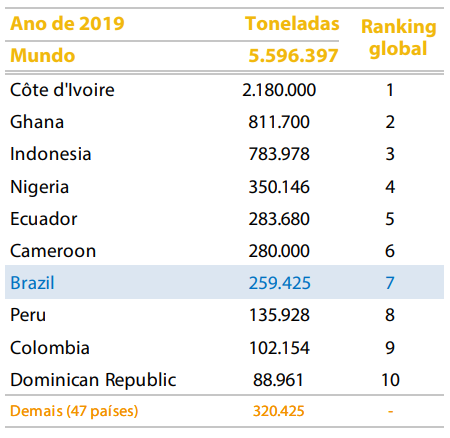
\includegraphics[scale=0.8]{../../Pictures/tabela.png} 
\label{fig2}
\legend{Fonte: \cite{8}}
\end{center}
\end{figure}

No Brasil o cultivo gera mais de 269 mil empregos diretos.

Segundo os dados do Ministério da Agricultura, a lavoura da amêndoa gerou R$\$$ 3,8 bilhões de valor bruto da produção agrícola (VBPA) em 2020, segundo os dados do Ministério da Agricultura, Pecuária e Abastecimento (MAPA). Os estados do Pará e da Bahia representaram 94$\%$ desse total. \cite{8}

\subsection{Dados Atuais}

A produção global de cacau atual é de aproximadamente 4.84M de toneladas, sendo a o continente africano o líder da produção 	com um market share de 76,1$\%$. \cite{8}

O Brasil é o sétimo maior produtor de cacau do mundo, sendo uma produção anual de 259.425 toneladas.

Segundo os dados do último Censo Agropecuário (2017), Há mais de 93 mil estabelecimentos produtores de cacau no País, sendo 69 mil na Bahia (74$\%$ do total) e 18 mil no Pará (19$\%$). \cite{8}

No Brasil o cultivo gera mais de 269 mil empregos diretos.

Segundo os dados do Ministério da Agricultura, a lavoura da amêndoa gerou R$\$$ 3,8 bilhões de valor bruto da produção agrícola (VBPA) em 2020, segundo os dados do Ministério da Agricultura, Pecuária e Abastecimento (MAPA). Os estados do Pará e da Bahia representaram 94$\%$ desse total. \cite{8}


\subsection{Avanços do processamento}

Antigamente o cacau era um privilégio da nobreza, porém atualmente com o avanço da tecnologia no processamento, o cacau se tornou amplamente utilizado pelo mundo todo. \cite{9}

Técnicas como a Conchagem (os ingredientes refinados recebem mais adição de gordura e emulsificante, formando uma massa fluida) e os maquinários possibilitaram a expansão da produção do chocolate. \cite{9}

\section{Matéria-prima}

O presente estudo tem como foco entender o processo de fabricação de chocolate através do cacau como matéria-prima. Analisando alguns dados sobre o cacau no mundo e no Brasil é possível afirmar que esse setor é muito promissor.

Atualmente a lavoura ocupa uma área de 617,5 mil hectares no País, e produz cerca de 310,5 mil toneladas, segundo o Instituto Brasileiro de Geografia e Estatística (IBGE). A maior área de plantio está na Bahia, com 440 mil hectares, 71,2$\%$ da área de cacau no País, o Pará é o maior produtor, com 146,4 mil toneladas numa área de 149,8 mil hectares. A produção baiana, por sua vez, é de 106 mil toneladas. Juntos somam 93$\%$ da produção nacional. \cite{6}

Uma das causas da grande produção dessa matéria-prima no país é o ambiente favorável, o cacaueiro (\textit{Theobroma cacao}) é uma frutífera tropical, originada da região amazônica.

Em relação aos métodos de produção do cacau foram identificados seis técnicas diferentes, e variações em dois desses métodos (Tabela \ref{table1}). Esses métodos apresentam uma gradação entre o plantio completamente exposto ao sol (corte e queima) até aquele contendo um sombreamento denso (cabruca). A categoria ‘outros métodos’ reúne os de menor relevância em termos de área cultivada e, por isso, não foi incluída na Tabela \ref{table1}. Esses seis métodos são descritos a seguir em seus respectivos contextos históricos, o que permite compreender sua origem e tentativa de diferenciação em relação às práticas correntes no momento da nova propositura. Assim, apresentam-se subdivididos em dois grandes períodos, caracterizados como o início de implantação da cacauicultura e o período de sua expansão e intensificação. \cite{10}

{\fontsize{5.8}{8}\selectfont
\begin{center}
\begin{longtable}[c]{c|c|c|c|c}
\caption{Principais métodos de implantação e manejo dos cacauais, seus procedimentos, vantagens e desvantagens.}
\label{table1}\\
\hline
\rowcolor[HTML]{EFEFEF} 
\textbf{\begin{tabular}[c]{@{}c@{}}Método \\ e suas variações\end{tabular}} &
  \textbf{\begin{tabular}[c]{@{}c@{}}Período provável \\ de implantação \\ do método\end{tabular}} &
  \textbf{\begin{tabular}[c]{@{}c@{}}Procedimentos\\ efetuados\end{tabular}} &
  \textbf{Vantagens} &
  \textbf{Desvantagens} \\ \hline
\endhead
%
Corte e queima &
  1746 &
  \begin{tabular}[c]{@{}c@{}}Corte de toda a vegetação\\ nativa, seguido da queima.\\ As sementes de cacau eram\\ plantadas diretamente no\\ campo sob a sombra de cultivos\\ temporários, como mandioca\\ e milho. Após a colheita, as\\ plantas de cacau eram mantidas\\ sem o sombreamento até que\\ surgissem árvores espontâneas\\ na área. Após sete a dez anos, o\\ sombreamento era removido e a\\ plantação, mantida a pleno sol\end{tabular} &
  \begin{tabular}[c]{@{}c@{}}Elevada \\ produtividade\\ nos primeiros \\ anos\end{tabular} &
  \begin{tabular}[c]{@{}c@{}}Destruição das substâncias\\ húmicas do solo; estresse\\ das jovens plantas de cacau\\ sem o sombreamento;\\ vigorosa emergência\\ de plantas espontâneas;\\ elevada demanda de\\ mão de obra; rápido\\ envelhecimento da\\ plantação\end{tabular} \\ \hline
\begin{tabular}[c]{@{}c@{}}Corte sem\\ queimada\\ (Variação do\\ método corte e\\ queima)\end{tabular} &
  \begin{tabular}[c]{@{}c@{}}Primeiras décadas\\ de 1900\end{tabular} &
  \begin{tabular}[c]{@{}c@{}}Os mesmos procedimentos\\ do método de corte e queima\\ eram efetuados, com exceção\\ da queimada da vegetação\\ derrubada\end{tabular} &
  \begin{tabular}[c]{@{}c@{}}Conservação\\ de substâncias\\ húmicas do solo\end{tabular} &
  \begin{tabular}[c]{@{}c@{}}A vegetação cortada\\ deixada no solo \\ atrapalhava a movimentação \\ dos trabalhadores\end{tabular} \\ \hline
Cabruca tradicional &
  \begin{tabular}[c]{@{}c@{}}Primeiras décadas\\ de 1900\end{tabular} &
  \begin{tabular}[c]{@{}c@{}}Corte da vegetação herbácea\\ e do estrato intermediário.\\ Raleamento da vegetação do\\ dossel dominante, poupando-se\\ do corte as árvores de maior\\ porte, com copa alta e folhagem\\ pouco densa. Na fase adulta\\ dos cacaueiros, raleava-se o\\ sombreamento por meio de\\ anelamento das árvores\end{tabular} &
  \begin{tabular}[c]{@{}c@{}}Conservação\\ de substâncias\\ húmicas do solo;\\ controle de plantas\\ espontâneas; rápido\\ desenvolvimento\\ dos cacaueiros;\\ conservação da\\ sociobiodiversidade;\\ economia em mão\\ de obra\end{tabular} &
  \begin{tabular}[c]{@{}c@{}}Queda de folhas, galhos\\ e árvores mortas sobre\\ os cacaueiros, podendo\\ danificá-los; baixa\\ produtividade\end{tabular} \\ \hline
\begin{tabular}[c]{@{}c@{}}Cabruca mantida\\ apenas no\\ sombreamento\\ provisório\\ (Variação do\\ método cabruca\\ tradicional)\end{tabular} &
  \begin{tabular}[c]{@{}c@{}}Primeiras décadas\\ de 1900\end{tabular} &
  \begin{tabular}[c]{@{}c@{}}Os mesmos procedimentos\\ do método cabruca tradicional\\ eram efetuados para a\\ formação do sombreamento. O\\ sombreamento era removido\\ após alguns anos do plantio dos\\ cacaueiros, ainda durante a fase\\ juvenil\end{tabular} &
  \begin{tabular}[c]{@{}c@{}}Conservação de\\ substâncias húmicas\\ do solo durante a fase\\ juvenil dos cacaueiros;\\ maior produtividade\\ dos cacaueiros\end{tabular} &
  \begin{tabular}[c]{@{}c@{}}Estresse das jovens\\ plantas de cacau sem o\\ sombreamento; rápido\\ envelhecimento da\\ plantação\end{tabular} \\ \hline
\begin{tabular}[c]{@{}c@{}}Intermediário\\ entre corte e\\ queima e cabruca\end{tabular} &
  \begin{tabular}[c]{@{}c@{}}Primeiras décadas\\ de 1900\end{tabular} &
  \begin{tabular}[c]{@{}c@{}}Derrubava-se a mata, poupando\\ do corte um número menor de\\ árvores em relação ao método\\ cabruca\end{tabular} &
  \begin{tabular}[c]{@{}c@{}}Fornecia\\ imediatamente o\\ sombreamento\\ definitivo, sem a\\ necessidade de\\ raleamentos futuros\end{tabular} &
  \begin{tabular}[c]{@{}c@{}}Queda de galhos mais\\ frequente em relação ao\\ que ocorre com a cabruca,\\ pois as árvores isoladas\\ eram menos resistentes ao\\ vento\end{tabular} \\ \hline
Derruba total &
  1964 &
  \begin{tabular}[c]{@{}c@{}}Roçagem da vegetação rasteira\\ e de toda a vegetação arbórea\\ nativa. Após 30-60 dias, efetuava-se \\ a queima da vegetação abatida.\\ Plantio de mudas de bananeira\\ para formação do sombreamento\\ provisório e de mudas de espécies\\ do gênero Erythrina para formação\\ do sombreamento definitivo,\\ com espaçamento de 24 x 24 m\\ (densidade de 25-30 árvores de\\ sombra por hectare)\end{tabular} &
  \begin{tabular}[c]{@{}c@{}}Elevada produtividade\\ nos primeiros anos de\\ cultivo\end{tabular} &
  \begin{tabular}[c]{@{}c@{}}Envelhecimento precoce\\ das plantações; entrada\\ em produção tardia; maior\\ custo de implantação\\ (quatro vezes mais caro em\\ comparação ao método\\ cabruca tradicional)\end{tabular} \\ \hline
\begin{tabular}[c]{@{}c@{}}Cabruca\\ tecnicamente\\ formada\end{tabular} &
  1978 &
  \begin{tabular}[c]{@{}c@{}}Execução das operações culturais\\ de acordo com os mesmos\\ critérios recomendados para\\ o método derruba total, com\\ exceção do preparo da área e do\\ raleamento do sombreamento.\\ A densidade do sombreamento\\ definitivo é de 25-30 árvores de\\ sombra por hectare\end{tabular} &
  \begin{tabular}[c]{@{}c@{}}Reduzida demanda\\ em capital, mão\\ de obra para a\\ implantação do\\ cacaual (economia\\ de 30\%) e tempo\\ na formação do\\ cacaual\end{tabular} &
  \begin{tabular}[c]{@{}c@{}}Queda de árvores\\ mortas e galhos sobre\\ os cacaueiros devido ao\\ raleamento\end{tabular} \\ \hline
\begin{tabular}[c]{@{}c@{}}Consórcio \\ cacau-seringueira\end{tabular} &
  \begin{tabular}[c]{@{}c@{}}Década de \\ 1980\end{tabular} &
  \begin{tabular}[c]{@{}c@{}}Plantio de cacaueiros nas\\ entrelinhas das seringueiras,\\ originalmente estabelecidas no\\ espaçamento de 7 x 3 m, com\\ densidade de aproximadamente\\ 450 cacaueiros por hectare\end{tabular} &
  \begin{tabular}[c]{@{}c@{}}As receitas econômicas\\ provenientes\\ da heveicultura\\ complementam as \\ receitas provenientes \\ da venda das \\ amêndoas de cacau\end{tabular} &
  \begin{tabular}[c]{@{}c@{}}Manejo das copas das\\ seringueiras de difícil\\ execução e custo elevado.\\ Pode haver sombreamento\\ excessivo para os\\ cacaueiros\end{tabular}
\end{longtable}
\centering \footnotesize{Fonte: \cite{10}}
\end{center}
}

\section{Produto}

\subsection{Importância Nutricional}
Segundo a Unimed \cite{unimed}, alguns benefícios podem ser elencados quando se fala do chocolate e esses são:

\begin{itemize}
\item O chocolate proporciona uma grande sensação de bem-estar
\item O consumo moderado de chocolate melhora o fluxo arterial 
\item Seu alto poder hidratante torna-o queridinho também no setor estético
\item Contribui para a saúde cerebral, reduzindo danos de acidente vascular cerebral
\item Reduz o estresse e alivia dores 
\item Melhora a saúde do coração
\item Estimula o sistema nervoso central
\item Diminui a sensação arterial
\item Protege a pele do sol
\item Diminui a fome
\end{itemize}

Mas pode-se elencar os benefícios por tipo de chocolate, o chocolate ao leite, chocolate meio amargo e amargo e chocolate branco.

O chocolate meio amargo e amargo são ótimos na circulação sanguínea, aumentam o colesterol bom, além de ser muito rico em alguns nutrientes, tais como o magnésio, ferro e selênio. O consumo moderado diário deste tipo de chocolate aumenta o metabolismo e reduz o apetite. \cite{saude}
	
Já o chocolate ao leite é o produto que tem menos gordura hidrogenada e por isso é o menos calórico.
	
Por fim, o chocolate branco tem uma característica principal de ter menos cafeina na sua composição e por oferecer mais energia ao corpo. \cite{saude}

% Please add the following required packages to your document preamble:
% \usepackage[table,xcdraw]{xcolor}
% If you use beamer only pass "xcolor=table" option, i.e. \documentclass[xcolor=table]{beamer}
% \usepackage{longtable}
% Note: It may be necessary to compile the document several times to get a multi-page table to line up properly
\begin{longtable}[c]{
>{\columncolor[HTML]{EFEFEF}}l |l|l}
\caption{Informações nutricionais do chocolate ao leite - 25g}
\label{table3}\\
\textbf{} & \cellcolor[HTML]{EFEFEF}\textbf{Quantidade por porção} & \cellcolor[HTML]{EFEFEF}\textbf{\% Valor diário} \\ \hline
\endhead
%
\textbf{Valor energético}   & 134 kcal  & 26,8 \% \\ \hline
\textbf{Carboidrato}        & 15 g      & 20,0 \%   \\ \hline
\textbf{Proteína}           & 1,2 g     & 6,4 \%  \\ \hline
\textbf{Gorduras totais}    & 7,7 g    & 56,0 \%   \\ \hline
\textbf{Gorduras saturadas} & 4,4 g    & 80,0 \%   \\ \hline
\textbf{Sódio}              & 11 mg     & 1,8 \% \\ \hline
\textbf{Colesterol}                  & 5,36 mg  &   0,9 \%  \\ \hline
\textbf{Fibra alimentar}             & 0,7 g     & 11,2 \% \\ \hline
\textbf{Cálcio}                      & 44,64 mg & 17,8 \% \\ \hline
\textbf{Ferro}                       & 0,36 mg   & 7,9 \% 
\end{longtable}
\begin{center}
\footnotesize{Fonte: \cite{fatsecret}}
\end{center} 
% Please add the following required packages to your document preamble:
% \usepackage[table,xcdraw]{xcolor}
% If you use beamer only pass "xcolor=table" option, i.e. \documentclass[xcolor=table]{beamer}
% \usepackage{longtable}
% Note: It may be necessary to compile the document several times to get a multi-page table to line up properly
\begin{longtable}[c]{
>{\columncolor[HTML]{EFEFEF}}l |l|l}
\caption{Informações nutricionais do chocolate meio amargo - 25g}
\label{table4}\\
\textbf{}                 & \cellcolor[HTML]{EFEFEF}\textbf{Quantidade por porção} & \cellcolor[HTML]{EFEFEF}\textbf{\% Valor diário} \\ \hline
\endhead
%
\textbf{Valor energético} & \cellcolor[HTML]{FFFFFF}131 kcal                       & \cellcolor[HTML]{FFFFFF}7\%                      \\ \hline
\textbf{Carboidrato}        & 14 g  & 5,0 \%  \\ \hline
\textbf{Proteína}           & 2 g   & 4,0 \%  \\ \hline
\textbf{Gorduras totais}    & 8,3 g & 15,0 \% \\ \hline
\textbf{Gorduras saturadas} & 5,4 g & 24,0 \% \\ \hline
\textbf{Sódio}              & 12 mg & 1,0 \%  \\ \hline
\textbf{Gorduras trans}              & 0 mg  &   -    \\ \hline
\textbf{Fibra Alimentar}             & 2 g   & 6,0 \%  \\ \hline
\textbf{Cálcio}                      & 35 mg & 4,0 \%  \\ \hline
\end{longtable}
\begin{center}
\footnotesize{Fonte: \cite{fatsecret}}
\end{center} 
% Please add the following required packages to your document preamble:
% \usepackage[table,xcdraw]{xcolor}
% If you use beamer only pass "xcolor=table" option, i.e. \documentclass[xcolor=table]{beamer}
% \usepackage{longtable}
% Note: It may be necessary to compile the document several times to get a multi-page table to line up properly
\begin{longtable}[c]{
>{\columncolor[HTML]{EFEFEF}}l |l|l}
\caption{Informações nutricionais do chocolate amargo - 25g}
\label{table5}\\
\textbf{}        & \cellcolor[HTML]{EFEFEF}\textbf{Quantidade por porção} & \cellcolor[HTML]{EFEFEF}\textbf{\% Valor diário} \\ \hline
\endhead
%
\textbf{Valor energético} & \cellcolor[HTML]{FFFFFF}131 kcal              & \cellcolor[HTML]{FFFFFF}7\%             \\ \hline
\textbf{Carboidrato}              & 13 g    & 4,0 \%   \\ \hline
\textbf{Proteína}                 & 2 g     & 3,0 \%   \\ \hline
\textbf{Gorduras totais}          & 9,2 g   & 17,0 \%  \\ \hline
\textbf{Gorduras saturadas}       & 5,8 g   & 26,0 \%  \\ \hline
\textbf{Sódio}                    & 5 mg    & 0,4 \% \\ \hline
\textbf{Gorduras trans}  & 0 mg    &    -    \\ \hline
\textbf{Fibra Alimentar} & 3 g     & 9,0 \%   \\ \hline
\textbf{Cálcio}          & 12,5 mg & 8,0 \%   \\ \hline
\end{longtable}
\begin{center}
\footnotesize{Fonte: \cite{fatsecret}}
\end{center} 

\subsection{Importância Ambiental}

A produção do cacau vem se tornando cada vez mais ESG com o tempo, dados da ONU dizem que houve um aumento de 8$\%$ na produção sustentável dos grãos de cacau entre 2017 e 2018, ou seja, a produção sustentável saiu de  36$\%$ em 2017 para 44$\%$ em 2018. \cite{xpeed}

Ao mesmo tempo, a indústria do chocolate também vem aumentando o direcionamento ESG com o tempo. Com as certificações de qualidade atualizadas, é possível saber qual produtor e fabricante tem um pensamento e uma produção sustentável ou não, com a ISO 9001:2015 é fácil realizar essa diferenciação. \cite{dengo}

\subsection{Importância Cultural}

A importância cultural do cacau se resume em 3 tópicos, são eles: o econômico, o histórico e o local.

Sobre a história do cacau, já foi abordado acima na introdução.

Sobre a importância de localização: O cacaueiro é uma planta nativa das bacias do rio Amazonas e rio Orinoco e tem a sua origem nas américas central e do sul. Para muitos povos havia até uma importância religiosa, como os Astecas. \cite{1}

Os próprios índios torravam e trituravam o fruto entre pedras para produzir um tipo de bebida típica, além disso, no Brasil, os maiores produtores do cacau estão localizados principalmente na Bahia e Pará, foi na Bahia que o cacau foi levado em meados do século XVIII. \cite{7}

Sobre a economia do cacau: No Brasil, o cacau é produzido em sua maioria em larga escala, sendo médios e grandes produtores. A concentração da produção se encontra principalmente na Bahia, Pará, Rondônia e Espírito Santo pelas características climáticas principalmente. No entanto, historicamente já passou por várias crises causando a redução da produção interna. \cite{8}

\newpage
\chapter{Mercado}
%\pagestyle{fancy}

Segundo a Associação Brasileira da Indústria de Chocolates, Amendoim e Balas (ABICAB). o brasileiro consumiu em 2020 11 bilhões de reais em chocolate, um crescimento de 1,5$\%$ comparado ao ano anterior. O presidente da associação, Ubiracy Fonseca, defende que a indústria de chocolates apresentou resultados muito consistentes para um ano tão atípico como foi 2020, e que os indicadores desse mercado apresentam potencial significativo para o crescimento do consumo interno e externo do setor. \cite{4}

\begin{figure}[H]
\begin{center}
\caption{Balança comercial de vendas de chocolates do Brasil em milhões de dolares}
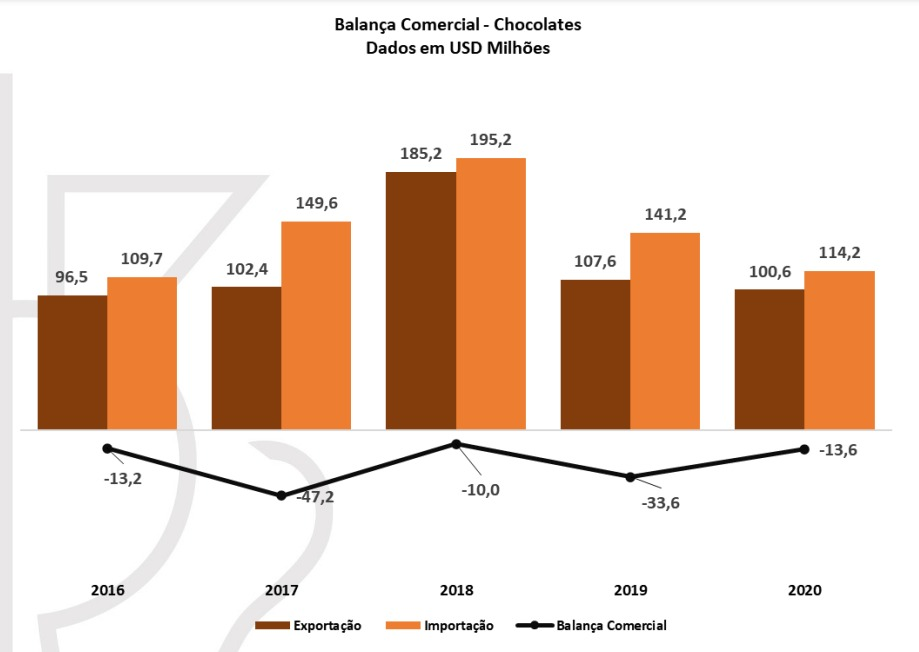
\includegraphics[scale=0.4]{../../Pictures/fig2.jpeg} 
\label{figmercado}
\legend{Fonte: \cite{4}}
\end{center}
\end{figure}

Analisando os números da KPMG, é possível concluir que a balança comercial do mercado de chocolate no brasil opera no negativo, ou seja, para que seja suprida a necessidade de chocolate no nosso país, foi importado 13 milhões de dólares a mais do que os valores de nossa exportação. Isso se dá pela falta de transformação da matéria prima em produto acabado levando em consideração que o país é o sétimo maior produtor de cacau do mundo. Esse número ainda é o menor dos últimos 5 anos, o que mostra que nossa indústria está em ascensão. \cite{forbes}

O chocolate ainda está presente em 82,6$\%$ dos lares brasileiros, um aumento de 9$\%$ percentuais comparado ao ano anterior. O avanço no consumo dos lares, juntamente com a grande necessidade de importação, resultou no aumento da produção de chocolate no último ano. \cite{4}

\begin{figure}[H]
\begin{center}
\caption{Gráfico comparativo entre produção, exportação e importação em volume}
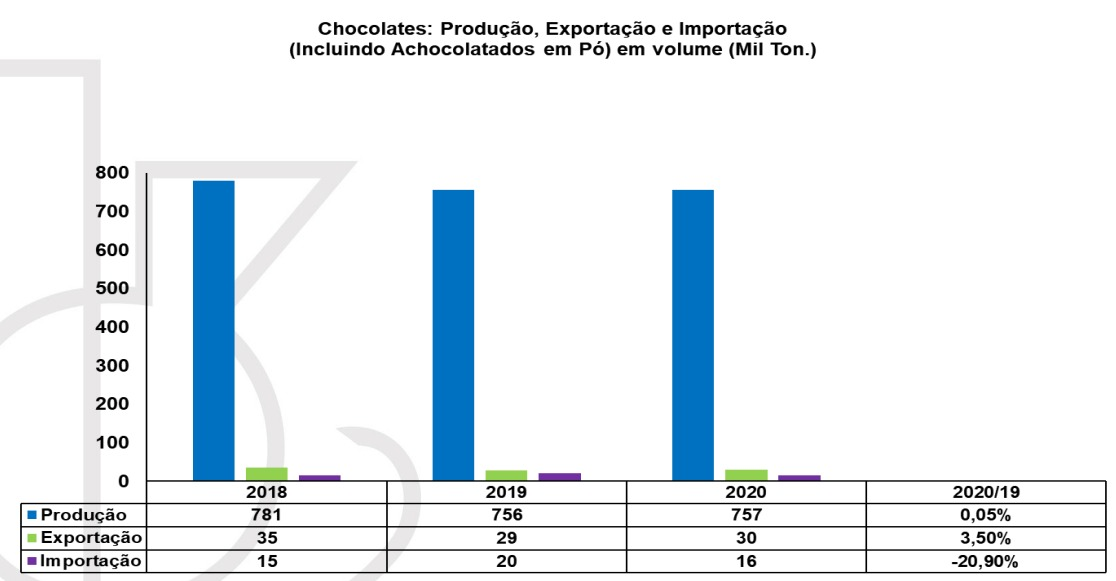
\includegraphics[scale=0.4]{../../Pictures/fig1.jpeg} 
\label{figmercado2}
\legend{Fonte: \cite{4}}
\end{center}
\end{figure}

\newpage
\chapter{Segmentação da Marca}

A empresa descrita neste trabalho foi caracterizada como produtora de chocolates especiais e foi criada a marca “Showcolate!”. A companhia se destaca pela preocupação com a sustentabilidade, qualidade dos produtos e pelo respeito com os colaboradores e clientes.

\begin{figure}[H]
\begin{center}
\caption{Logo da marca Showcolate!}

\includegraphics[scale=0.5]{logoShow.jpeg} 
\legend{Fonte: Autoria Própria}
\end{center}
\end{figure}

Com uma proposta de trazer inovação e uma explosão de sabores, a marca traz para o mercado não somente o processamento do cacau \textit{bean to bar}, mas também um propósito de mudar a maneira como o chocolate é consumido no Brasil e no mundo. Outro diferencial da empresa é o foco no mercado digital, assim será possível abranger clientes em diferentes centros urbanos do Brasil. 

A definição do público alvo para um plano de negócios como este da marca do showcolate é de extrema importância para assim conseguir ter o nos problemas e necessidades específicas desse tipo de grupo social. O público alvo em si, representa um segmento de pessoas e consumidores com hábitos e características que estão em comum, ou seja, uma parcela da população pela qual a empresa está focada.

A seguir está representado o público alvo da marca Showcolate!:

% Please add the following required packages to your document preamble:
% \usepackage[table,xcdraw]{xcolor}
% If you use beamer only pass "xcolor=table" option, i.e. \documentclass[xcolor=table]{beamer}
\begin{center}
% Please add the following required packages to your document preamble:
% \usepackage[table,xcdraw]{xcolor}
% If you use beamer only pass "xcolor=table" option, i.e. \documentclass[xcolor=table]{beamer}
\begin{table}[H]
\centering
\caption{Definição do público alvo}
\label{publico}
\begin{tabular}{
>{\columncolor[HTML]{EFEFEF}}l l}
\multicolumn{2}{c}{\cellcolor[HTML]{EFEFEF}{\color[HTML]{202124} \textbf{Definição do público alvo}}}                                                                                                                                    \\ \hline
\multicolumn{1}{l|}{\cellcolor[HTML]{EFEFEF}{\color[HTML]{202124} \textbf{Geografia}}}             & {\color[HTML]{202124} Principalmente em grandes centros}                                                                            \\ \hline
\multicolumn{1}{l|}{\cellcolor[HTML]{EFEFEF}{\color[HTML]{202124} \textbf{Sexo}}}                  & {\color[HTML]{202124} 70\% Mulheres e 30\% Homens}                                                                                  \\ \hline
\multicolumn{1}{l|}{\cellcolor[HTML]{EFEFEF}{\color[HTML]{202124} \textbf{Idade}}}                 & {\color[HTML]{202124} entre 30 a 75 anos}                                                                                           \\ \hline
\multicolumn{1}{l|}{\cellcolor[HTML]{EFEFEF}{\color[HTML]{202124} \textbf{Ocupação}}}              & {\color[HTML]{202124} Gerente ou Head ou Diretor de multinacionais}                                                                 \\ \hline
\multicolumn{1}{l|}{\cellcolor[HTML]{EFEFEF}{\color[HTML]{202124} \textbf{Uso}}}                   & {\color[HTML]{202124} Consumo próprio ou destinado para presente}                                                                   \\ \hline
\multicolumn{1}{l|}{\cellcolor[HTML]{EFEFEF}{\color[HTML]{202124} \textbf{Benefícios procurados}}} & {\color[HTML]{202124} Chocolate com alta qualidade}                                                                                 \\ \hline
\multicolumn{1}{l|}{\cellcolor[HTML]{EFEFEF}{\color[HTML]{202124} \textbf{Concorrência}}}          & Kopenhagen e Lindt                                                                                                                  \\ \hline
\multicolumn{1}{l|}{\cellcolor[HTML]{EFEFEF}{\color[HTML]{202124} \textbf{Lealdade da marca}}}     & {\color[HTML]{202124} \begin{tabular}[c]{@{}l@{}}Extremamente comprometidos com a marca, \\ não faz diferença o preço\end{tabular}}
\end{tabular}
\end{table}
\centering \footnotesize{Fonte: Autoria própria}
\end{center}

O nicho que representa os maiores clientes da marca, são mulheres ,casadas e com uma renda mensal acima de R\$7.000,00. Já o nicho de mercado que é mais lucrativo são pessoas jurídicas que realizam compras em grandes quantidades. Quanto aos potenciais clientes mais atrativos para a marca, são as pessoas abaixo de 35 anos que possuem renda familiar acima de R\$7.000,00 e realizam compras pela internet com alta frequência. 

E por fim, os clientes que se encaixam em em um grupo lógico, se assemelhando muito ao público alvo, são tais clientes da classe social A1, A2 e B1, que moram em grandes centros urbanos, tem mais de 30 anos e tem a vida muito estável em todos os âmbitos.

Além disso, foi estabelecido o organograma da Showcolate!, sendo 6 diretores os cargos mais altos e responsáveis pelo gerenciamento completo da marca, e alguns cargos menores para trabalhos mais específicos.

\begin{figure}[H]
\begin{center}
\caption{Organograma da Showcolate!}
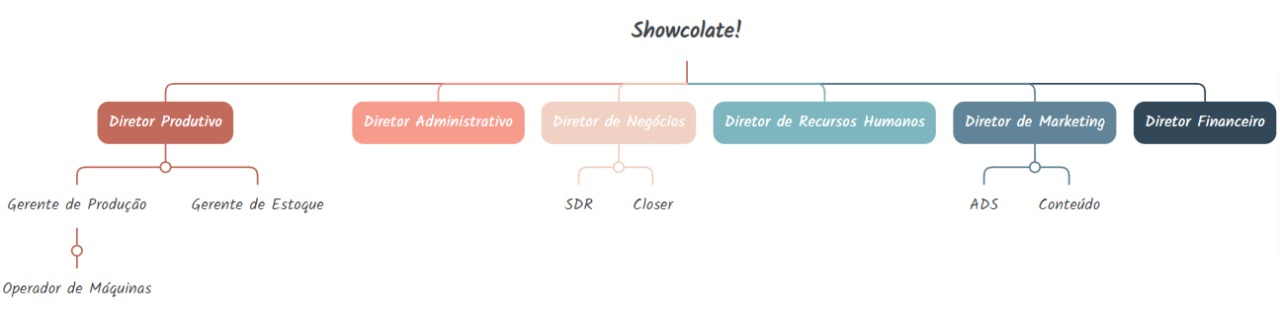
\includegraphics[scale=0.34]{org.jpeg} 
\label{-}
\legend{Fonte: Autoria própria}
\end{center}
\end{figure}


\newpage
\chapter{Análise Ambiental e Interna}

O setor do chocolate vive em constante mudança e evolução já que se trata de um produto que é consumido na maioria dos lares do país, e por isso precisa sempre se moldar de acordo com a vontade e o desejo dos seus consumidores. Dessa forma sempre acabam surgindo diversos produtos inovadores e para fabricá-los a indústria precisa estar preparada e ser bastante flexível.

Atualmente o mercado de chocolate está se voltando para produtos mais saudáveis e com maior teor de cacau, e também para produtos sem ingredientes de origem animal, já que uma das tendências atuais é o veganismo. Isso faz com que as empresas se preocupem mais com as matérias-primas utilizadas e também com embalagens mais chamativas e muitas vezes até mesmo sustentáveis, outra tendência atual do mercado que impacta o setor de chocolates.

A marca Showcolate! se preocupa muito com a qualidade dos seus produtos e para conseguir atender as tendências possui o chocolate amargo 70$\%$ que é mais saudável pelo seu alto teor de cacau e ainda assim saboroso e com sabores complexos, e o chocolate meio amargo 50$\%$ que além de possuir uma também alta concentração de cacau é vegano e possui a proposta de conquistar quem prefere chocolates mais suaves. Além disso, a empresa também possui a linha de chocolates maturados, que são chocolates especiais 70$\%$ armazenados durante um longo período para refinar aromas e sabores, e que segue a tendência do mercado de produtos mais exclusivos e premium. Assim, a empresa consegue alcançar diferentes públicos e conquistar cada vez mais pessoas.

É de extrema importância se entender as tendências do cliente para o futuro de curto, médio e longo prazo, caso uma empresa tenha a ambição de passar pelo filtro do tempo.
	
	As tendências do cliente são diversas e são as seguintes: tendências comportamentais, de estilo de vida, de gostos tais como moda e tendências culturais. Atualmente, as tendências comportamentais para alimentos são cada vez a maior procura de uma alimentação saudável, livre de gorduras e mais fitness, além disso as pessoas estão procurando cada vez mais opções de alimentos produzidos por empresas ESG, que tenham esse selo, ou seja, empresas que tenham consciência ambiental, social e governamental, além disso, as tendências culturais e comportamentais foram se moldando e mudando com o surgimento da pandemia, influenciando também no modo como as pessoas consomem e também sua intensidade, por fim mas não menos importante, há uma forte tendência ao veganismo, ou seja, produtos que não tenham ingredientes com origem animal. 
	
	Tudo isso tem uma implicação prática que não se pode deixar de lado. Com o advento das ondas fitness, o consumo de chocolate pode diminuir, além disso, empresas que não são ESG podem ver o resultado operacional e de vendas derreter num futuro próximo, e por fim já que a maneiro como as pessoas consomem mudou, a maneira como as vendas ocorrem precisa ser modificada para acompanhar essas tendências, atualmente as vendas online dispararam e vão permanecer alta mesmo com a volta do presencial, e isso deve ser acompanhado pelas empresas.
	
	Analisando as tendências demográficas, a maioria delas não irá afetar o modelo de negócios da empresa em questão (a Showcolate), já que as vendas ocorrem de maneira digital ou online, facilitando a quebra de várias barreiras demográficas e além disso, a diversidade de produtos da empresa consegue atender de forma tanto generalista quanto personalizada as diversas regiões do brasil, mitigando as implicações da tendência demográfica.
	
	Abordando de forma mais detalhista o tópico comentado à dois parágrafos, os dados de risco retorno para investimentos de “ser verde” ou para se tornar uma empresa ESG são muito promissores, isso devido às tendências tanto de consumo quanto culturais da sociedade global, isso se mostra como verdade quando fundos de venture capital focados em crescimento e retornos agressivos estão voltando o foco para empresas com os princípios de sustentabilidade e ESG.

A showcolate tem o foco a médio prazo no mercado brasileiro e para este mercado, como a taxa base atual está em 13,75$\%$, todas as iniciativas empreendedoras perdem força, já que para fazer sentido o investimento em empresas, é necessário superar esta taxa. As projeções econômicos no entanto são positivas, uma vez que para 2023 a tendência é de redução da taxa selic, com uma inflação retraindo e em alguns casos recentes até uma deflação, afetando positivamente o fluxo de caixa descontado.
	
	A seguir um gráfico das taxas de juros históricas no Brasil:

\begin{figure}[H]
\begin{center}
\caption{Taxa SELIC}
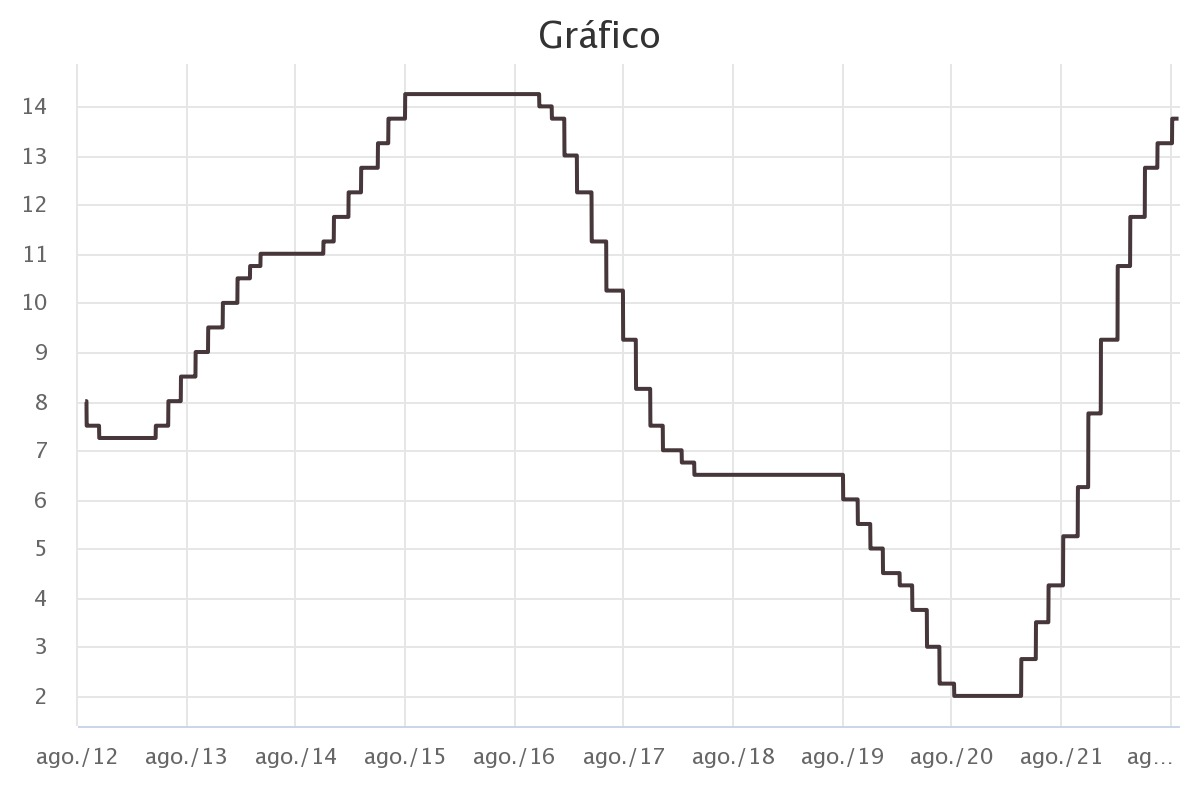
\includegraphics[scale=0.2]{WhatsApp Image 2022-08-25 at 20.37.35 (1).jpeg} 
\legend{Fonte: Banco Central}
\end{center}
\end{figure}


Como é possível verificar no gráfico, as taxas de juros no Brasil está quase no teto, com tendência de baixa para o futuro

	É possível que a regulamentação para o percentual de ingredientes para cada tipo de produto seja modificado, uma vez isso acontecendo, iria afetar a precificação dos produtos afetados por esta mudança, podendo ser um aumento ou diminuição no preço final, ou seja, a margem de lucro pode diminuir ou o preço final aumentar, gerando perda de clientes da base.

	Politicamente os possíveis riscos são de alguma sanção ou adição de leis.

	Além disso, a pandemia mudou muitos quesitos e tendências comportamentais da sociedade brasileira, que deve ser seguida pela Showcolate para otimizar ainda mais os resultados e não ficar para trás da concorrência. As implicações no planejamento estratégico foi a seguinte:

\begin{itemize}
\item Setor comercial: Mudança na maneiro como faz-se as vendas. Normalmente o modelo de negócios de uma empresa de chocolates, para crescimento é por meio do franqueamento, como ocorre com a cacau show ou com a kopenhaguen, no entanto devido também às mudanças devido à pandemia o modelo de expansão da showcolate se fez por meio das vendas online.
\end{itemize}

A visão da Showcolate! é alcançar o topo da qualidade e comercialização no mercado brasileiro de chocolates especiais com alto teor de cacau em 5 anos. E a missão da empresa é transformar a produção de chocolate em um processo mais sustentável e saudável para os consumidores, buscando os melhores sabores e desenvolvendo o mercado consumidor. Para isso, a companhia definiu os seguintes valores:

\begin{itemize}
\item Qualidade superior;
\item Sustentabilidade;
\item Respeito com os colaboradores e clientes.
\end{itemize}

A empresa mesmo não possuindo um grande investimento em P$\&$D, entende e acompanha as necessidades dos seus clientes e consegue ser inovadora. E além disso, também possui muitos outros aspectos que a engrandecem como sua preocupação com ingredientes de alta qualidade e a sustentabilidade dentro da empresa. A Showcolate! por focar no mercado online consegue alcançar clientes de todo o canto do país, mas isso também pode ser uma fraqueza, visto que atualmente muitas pessoas ainda não estão acostumadas a comprar chocolates pela internet. No entanto, a companhia está focada em auxiliar no crescimento desse mercado com um marketing agressivo e altos investimentos para conquistar o público alvo da empresa.
	
Outro ponto que a empresa também precisa trabalhar com muito cuidado é sua carteira de fornecedores, pois a confiabilidade e a constância da entrega de um bom produto depende também das mesmas qualidades advindas do fornecedor. Isso impacta principalmente os chocolates maturados, que deverão possuir uma boa gestão de estoque e demanda para que possam ser vendidos durante o ano todo sem muitas preocupações.

Análise SWOT da empresa:

\begin{itemize}
\item Fraquezas
\subitem Menor apelo emocional: Chocolate é um produto que gera satisfação e prazer ao consumidor e por esse motivo muitas vezes sua compra vem de um impulso, quando o consumidor se depara com uma loja de chocolates ou com um chocolate na prateleira de um mercado. No caso da venda online esse apelo é menor, já que o consumidor precisa buscar o site e esperar a entrega.
\subitem Maior preocupação com embalagem e entrega: chocolate além de ser bom faz parte da sua qualidade ter também uma boa aparência, o que pode ser um risco no caso de vendas por internet considerando que podemos ter problemas com temperatura ou danos mecânicos.
\item Forças
\subitem Fácil acesso e distribuição: No ramo de chocolates premium os concorrentes tem atualmente uma estratégia de lojas próprias, que na maioria das vezes localiza-se em shoopings ou bairros de maior poder aquisitivo. O produto vendido pela internet torna-se mais democrático e pode até chegar a atingir outras classes sociais.
\subitem Qualidade: O chocolate da Showcolate além de ser do tipo premium (que não tem estratégia de produção em massa) é focado apenas em três tipos de chocolates com foco total em qualidade do produto e do processo.
\item Ameaças
\subitem Baixa barreira de entrada: Nesse ramo já existem grandes marcas consolidadas no segmento, que apesar de nos diferenciarmos dessas marcas por alguns aspectos esses grandes representantes do mercado podem mudar rapidamente de estratégia pela facilidade de investimento.
\subitem Incerteza de demanda:  A venda pela internet além de ser uma modalidade nova para produtos como o chocolate é um tipo de venda que permite a devolução do produto com um prazo de tempo maior. Por isso a incerteza nas vendas iniciais pode ser muito grande
\item Oportunidades
\subitem Ganho de mercado novo: Hoje em dia não encontramos nenhum chocolate do tipo premium e nem dos outros segmentos sendo vendidos pela internet, o que pode proporcionar um crescimento rápido nessa área e tornar-se uma referência.
\subitem Foco em qualidade: Com o mix de produtos muito baixo podemos focar totalmente na qualidade e criar cada vez mais uma identificação da marca pelo consumidor 
\end{itemize}


\newpage
\chapter{Qualidade}

Os chocolates produzidos pela Showcolate visam o reconhecimento principalmente através da sua qualidade e sabor inconfundível, por isso o foco maior da gestão da qualidade é voltado para o produto. Com o grande objetivo de produzir chocolates em barra com alto teor de cacau e padrão de qualidade elevado (categoria premium de chocolates). Entretanto, a empresa conta com outros dois diferenciais, ligado ao processo de produção e ao usuário final.

O grande diferencial e fator de qualidade relacionado ao processo são suas conformidades com as normas ambientais de produção, caracterizando assim a empresa como sustentável e preocupada com o meio ambiente, o que além de trazer o benefício claro de sustentabilidade também contribui para a agregação de valor ao produto através da consciência ambiental dos consumidores.

Em relação ao usuário a empresa é uma das poucas que tem como canal de vendas o meio digital, facilitando assim o acesso aos usuários e a comodidade de entregas agendadas.

A Showcolate tem como foco estar em conformidade com a ISO 9001 para desenvolvimento e padronização de processos produtivos e também gerenciais. Desse modo, será possível manter a qualidade dos produtos sempre alta e padronizada, melhorando assim a satisfação dos clientes com relação aos chocolates. E além desse sistema de gestão é interessante para a empresa também estar condizente com a norma ISO 14001, já que a Showcolate possui essa vertente mais sustentável e pretende diminuir ao máximo seu impacto no planeta. Assim, a marca terá diversos benefícios tanto pela padronização dos processos quanto pela sustentabilidade que irá alcançar obedecendo as duas ISOs. Um começo estruturado em conjunto com a visão de sempre evoluir será um ponto chave para o sucesso da Showcolate.


Para os produtos oferecidos pela Showcolate são dois os principais elementos de qualidade buscados:

\begin{itemize}
\item Conformidade: as barras de chocolates produzidas são dividas em quatro tipos, que seguem uma receita rigorosa de porcentagens de ingredientes para que suas características sejam percebidas pelo consumidor. Além disso todo o processo é seguido de forma que não haja erros no produto final entregue ao cliente, conferindo assim as características prometidas pelo produto (premium de alta qualidade) e alinhado com as expectativas do cliente.
\item Estética: Os produtos seguem a linha premium não apenas no sabor, mas também em sua apresentação. A aparência das barras de chocolate e sua embalagem são estaticamente pensadas para agradar os clientes e além disso cumprem com uma função muito utilizada na compra de chocolates que é o uso para presentes.
\end{itemize}



\newpage
\chapter{Análise de Concorrentes}

O mercado de chocolate, mesmo em constante crescimento e mudança, possui marcas bem definidas e conhecidas em cada segmento do mesmo. E é importante notar que algumas empresas mesmo possuindo produtos similares podem acabar não disputando o mesmo público-alvo devido a estratégia da marca. Na figura a seguir são mostrados os 3 principais grupos estratégicos do setor:

\begin{figure}[H]
\begin{center}
\caption{Grupos estratégicos do mercado de chocolate}
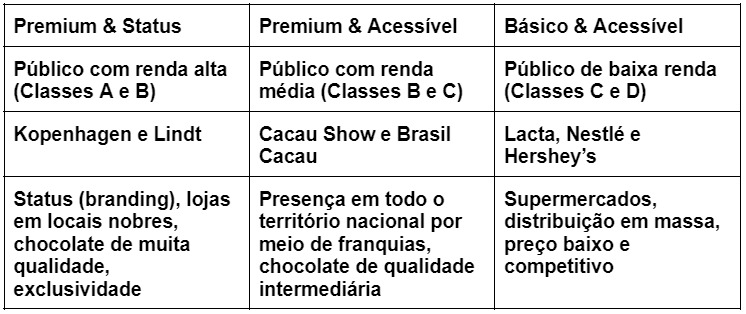
\includegraphics[scale=0.5]{WhatsApp Image 2022-08-19 at 19.04.28.jpeg} 
\legend{Fonte: Autoria Própria}
\end{center}
\end{figure}

A maior parte do mercado de chocolates no Brasil é composto por empresas identificadas no terceiro grupo (Básico $\&$ Acessível). Essas empresas por estratégia tem seus produtos mais difundidos aos consumidores por meio de canais de distribuição em massa (mercados por todo o país). Já as empresas listadas dentro dos dois primeiros grupos (Premium e premium acessível) representam uma pequena parte do mercado e se dividem basicamente entre Cacau Show e Kopenhagen que representam respectivamente 70$\%$ e 30$\%$ do mercado de chocolates finos do Brasil.

Quando olhamos para participação geral no mercado de chocolates brasileiro as companhias líderes são: Mondelez (Diamante Negro, Bis e Sonho de Valsa, etc) com 32$\%$, Garoto com 23$\%$, Nestlé com 21$\%$ e Hersheys com 4$\%$.

Participação de mercado das maiores empresas do ramo de chocolates no Brasil: 

\begin{figure}[H]
\begin{center}
\caption{Participação no mercado}
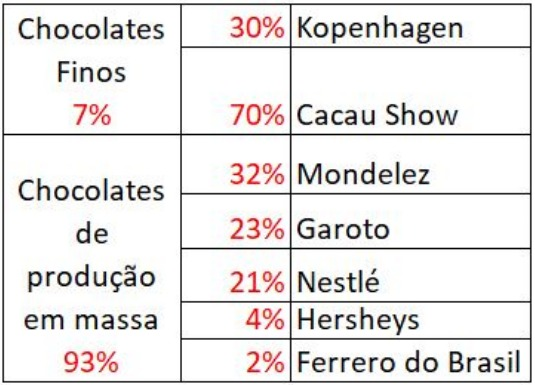
\includegraphics[scale=0.4]{concorrentes.jpeg} 
\legend{Fonte: Autoria Própria}
\end{center}
\end{figure}

\begin{itemize}
\item Grupo Premium $\&$ Status
\subitem Este grupo detém uma grande fatia do mercado de produtos finos, e por serem os concorrentes diretos isso afeta de forma negativa a showcolate, uma vez que é um mar vermelho esse segmento de atuação. As duas empresas do grupo detém o monopólio quase que total do nicho de mercado.
\subitem Quanto às integrações, por serem empresas muito grandes, ambas detém um controle tanto da integração para frente, quando para trás.
\subitem Ambas as empresas vem crescendo tanto em franquias quanto em ativos.
\item Premium $\&$ Acessível
\subitem Este grupo detém grande parte da produção e venda de produtos em massa.
\subitem Já quanto a intefração para frente e para trás, a maioria das empresas também detém tal expertise.
\subitem Relativo aos ativos e competências, existem ressalvas para cada concorrente, por não serem o nicho de mercado foco dos produtos da showcolate.
\item Básico $\&$ Acessível
\subitem Quanto a expansão de mercado este grupo apresenta o menos risco para a showcolate, justamente por ser um dos grupos que menos se equipara com a empresa, justamente por não atacar a mesma persona.
\subitem As integrações acontecem de forma tangencial.
\subitem E não existem muitas estratégias ofensivas mapeadas.
\end{itemize}

As empresas integrantes do primeiro grupo (Premium) caracterizam-se por focar no sabor único dos seus chocolates e consequentemente na sua qualidade. Assim como agregar valor a sua marca através de estratégias de branding e exclusividade dos seus produtos voltados a um público de maior poder aquisitivo. Dessa forma as empresas desse grupo também têm uma estrutura de custos muito maior, que envolve um maior detalhe na escolha de fornecedores, processo e até na distribuição.

O segundo grupo (Premium acessível) tem uma estratégia de alcance maior que os do primeiro grupo, focando na qualidade do seu produto, mas também preocupado em atender em diversas localidades através de franquias espalhadas em todo o Brasil. Aqui a estratégia é também ter qualidade, mas com padronização e distribuição em maior escala através das lojas oficias em forma de franquias.

No terceiro grupo (Acessível) temos empresas com foco em volume e custos competitivos. Essas empresas não apresentam lojas próprias, sua estratégia e atingir o público em larga escala através de mercados, supermercados, padarias, etc. Assim para esse grupo a competição por preço e atenção do público é essencial.

Para os pontos fortes, serão avaliados os pontos fortes e fracos de cada concorrente para cada um dos parâmetros, sendo eles:
\begin{itemize}
\item Qualidade do produto
\item Qualidade do serviço
\item Participação de mercado
\item Reconhecimento/Posicionamento de arca e
\item Satisfação dos clientes
\end{itemize}
Os que mais se destacaram por estarem acima da média em mais de um desses quesitos foram as empresas da Kopenhagen, Lindit e Cacau Show.

A seguir está uma matriz representando a comparação entre os parâmetros estudados:

\begin{figure}[H]
\begin{center}
\caption{Matriz dos concorrentes}
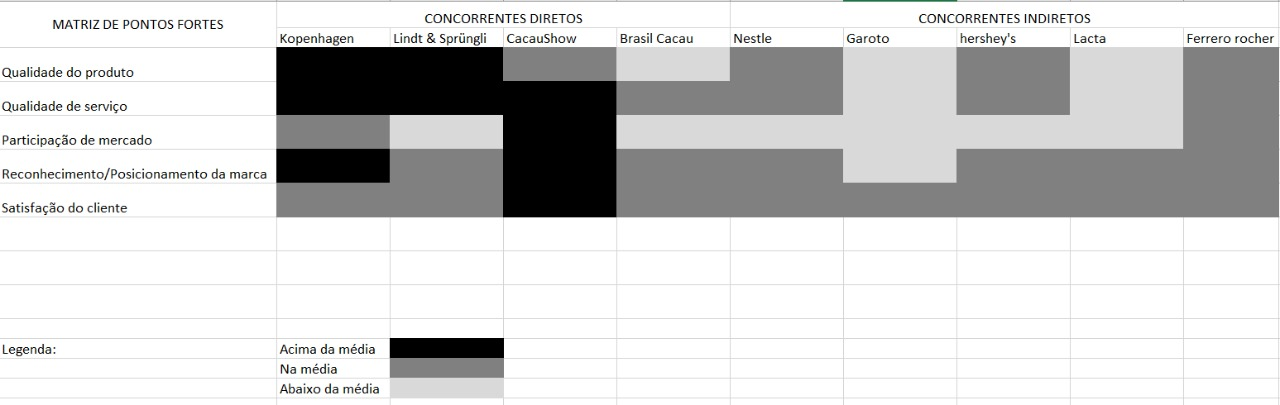
\includegraphics[scale=0.3]{concorrentes2.jpeg} 
\legend{Fonte: Autoria Própria}
\end{center}
\end{figure}

\begin{figure}[H]
\begin{center}
\caption{Grupos estratégicos e suas características}
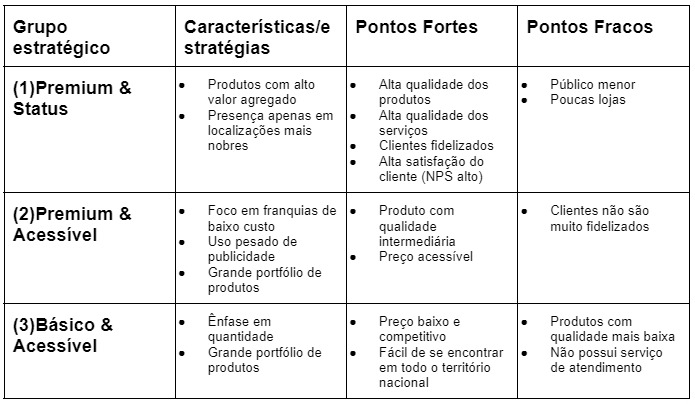
\includegraphics[scale=0.5]{WhatsApp Image 2022-08-19 at 18.59.03.jpeg} 
\legend{Fonte: Autoria Própria}
\end{center}
\end{figure}

\newpage
\chapter{Normas e Leis Regulamentadoras}
%\pagestyle{fancy}

O setor alimentício possui leis e normas bem definidas e detalhadas pela Agência Nacional de Vigilância Sanitária (Anvisa). Essa organização, segundo artigo 8º da Lei n. 9782/99 \cite{anvisa9782}, deve: “regulamentar, controlar e fiscalizar os produtos e serviços que envolvam risco à saúde pública”. Então será principalmente por meio dela que a empresa deve se informar para que esteja condizente com a legislação e normas vigentes. 

A principal preocupação desse setor é com relação às condições higiênicos-sanitárias, pois engloba todo o processo de fabricação, desde o recebimento das matérias-primas até o transporte final do produto acabado. Logo, a empresa deve se atentar principalmente à PORTARIA Nº 326 postada em 1997 \cite{anvisa326} que menciona o seguinte objetivo: “O presente Regulamento estabelece os requisitos gerais (essenciais) de higiene e de boas práticas de fabricação para alimentos produzidos/fabricados para o consumo humano.” 

Além disso, é importante estar de acordo com a legislação e os projetos de lei que existem para criação do produto, para planejar sua composição e marca e que consiga atender a todos os requisitos e possa ser comercializado sem problemas. Nesse sentido, os produtos que serão comercializados pela empresa são: chocolate amargo, chocolate meio-amargo e chocolate ao leite que devem obedecer a RESOLUÇÃO DE DIRETORIA COLEGIADA - RDC N° 264, de 2005 \cite{anvisa264}. Contudo, já existe o Projeto de Lei n° 1769, de 2019 \cite{anvisa1769} que pode influenciar nos requisitos relacionados à composição do chocolate.  

Por fim, ainda existem os requisitos relacionados ao modo como o produto será embalado e detalhes que necessitam estar nos rótulos de cada produto. Segundo a RESOLUÇÃO DE DIRETORIA COLEGIADA - RDC Nº 91, de 2001 \cite{anvisa91}, as embalagens, da mesma forma que os equipamentos que entram em contato com alguma parte do produto, devem manter o alimento protegido de fatores externos e não podem interferir ou mudar suas características. Existe uma classificação de embalagens de acordo com o tipo de material que é utilizado, e cada um deles possui um regulamento específico. Os rótulos, no entanto precisam estar de acordo com a RESOLUÇÃO DE DIRETORIA COLEGIADA – RDC Nº 259, de 2002 \cite{anvisa259} e RDC Nº 360, de 2003 \cite{anvisa360}, no quesito de informações obrigatórias que devem constar nos rótulos. Também é importante acompanhar a nova RDC Nº 429, de 2020 \cite{anvisa429}, que já está entrando em vigência e também a RDC N° 26, de 2015 \cite{anvisa26}, que torna obrigatória a lista em destaque dos ingredientes alergênicos.     

Essa parte é de demasiada importância para que a empresa não tenha problemas na comercialização dos produtos fabricados e também consiga manter a qualidade das operações durante todo o processo produtivo para que o produto chegue ao cliente com alta qualidade. Por isso é interessante que a empresa, além de seguir os requisitos técnicos e regulamentações, consiga também atender às boas práticas, garantindo por meio disso uma qualidade ainda mais elevada.

{\fontsize{8.8}{12}\selectfont
\begin{center}
% Please add the following required packages to your document preamble:
% \usepackage[table,xcdraw]{xcolor}
% If you use beamer only pass "xcolor=table" option, i.e. \documentclass[xcolor=table]{beamer}
% \usepackage{longtable}
% Note: It may be necessary to compile the document several times to get a multi-page table to line up properly
\begin{longtable}[c]{
>{\columncolor[HTML]{EFEFEF}}l |lll}
\caption{Principais regulamentações para chocolate amargo, meio-amargo e ao leite}
\label{table2}\\
\cline{2-4}
\textbf{} &
  \multicolumn{1}{l|}{\cellcolor[HTML]{EFEFEF}\textbf{Chocolate amargo}} &
  \multicolumn{1}{l|}{\cellcolor[HTML]{EFEFEF}\textbf{Chocolate meio-amargo}} &
  \cellcolor[HTML]{EFEFEF}\textbf{Chocolate ao leite} \\ \hline
\endhead
%
\textbf{\begin{tabular}[c]{@{}l@{}}Características \\ do produto\end{tabular}} &
  \multicolumn{1}{l|}{\begin{tabular}[c]{@{}l@{}}De acordo com o projeto \\ de lei Projeto de Lei \\ 1769/2019 é definido \\ que “chocolate amargo: \\ chocolate contendo o \\ mínimo de 35\% de \\ sólidos totais de cacau, \\ dos quais ao menos \\ 18\% devem ser de \\ matéria gorda de cacau, \\ proveniente da manteiga \\ de cacaue da massa de \\ cacau e outros \\ ingredientes, e 14\% devem \\ ser de sólidos totais de cacau \\ isenta de gordura”.\end{tabular}} &
  \multicolumn{1}{l|}{\begin{tabular}[c]{@{}l@{}}De acordo com o projeto \\ de lei Projeto de Lei \\ 1769/2019 é definido \\ que “chocolate meio \\ amargo: chocolate \\ contendo o mínimo de \\ 35\% de sólidos totais \\ de cacau, dos quais ao \\ menos 18\% devem ser \\ de matéria gorda de \\ cacau, proveniente da \\ manteiga de cacau e da \\ massa de cacau e outros \\ ingredientes, e 14\% devem \\ ser de sólidos totais de \\ cacau isenta de gordura”.\end{tabular}} &
  \begin{tabular}[c]{@{}l@{}}De acordo com o projeto \\ de lei Projeto de Lei \\ 1769/2019  é definido \\ que “chocolate ao leite: \\ chocolate contendo \\ o mínimo de 27\% de \\ sólidos totais de cacau \\ e outros ingredientes, \\ e o mínimo de 14\% de \\ sólidos totais de leite \\ oriundo da evaporação \\ parcial ou total de leite \\ inteiro, de leite parcial \\ ou totalmente desnatado, \\ de nata parcial ou totalmente \\ desidratada, de manteiga \\ ou de matéria gorda láctea \\ e outros derivados de leite”.\end{tabular} \\ \hline
\textbf{\begin{tabular}[c]{@{}l@{}}Especificações \\ de equipamentos\end{tabular}} &
  \multicolumn{3}{l}{\begin{tabular}[c]{@{}l@{}}De acordo com as definições do PORTARIA Nº 326, DE 30 DE JULHO \\ DE 1997 da Agência Nacional de Vigilância Sanitária – ANVISA - \\ “4.5.2 Equipamentos e recipientes: Os equipamentos e os recipientes que são utilizados\\  nos diversos processos produtivos não devem constituir um risco à saúde. \\ Os recipientes que são reutilizáveis devem ser fabricados de material que permita \\ a limpeza e desinfeção completa. Uma vez usados com matérias tóxicas não devem \\ ser utilizados posteriormente para alimentos ou ingredientes alimentares sem que \\ sofram desinfeção”\end{tabular}} \\ \hline
\textbf{\begin{tabular}[c]{@{}l@{}}Especificações \\ de armazenagem\end{tabular}} &
  \multicolumn{3}{l}{\begin{tabular}[c]{@{}l@{}}De acordo com as definições do PORTARIA Nº 326, DE 30 DE JULHO \\ DE 1997 da Agência Nacional de Vigilância Sanitária – ANVISA - \\ “3.3. Armazenamento: é o conjunto de atividades e requisitos para se \\ obter uma correta conservação de matéria-prima, insumos e produtos acabados. ”\end{tabular}} \\ \hline
\textbf{\begin{tabular}[c]{@{}l@{}}Especificações \\ de rótulo\end{tabular}} &
  \multicolumn{3}{l}{\begin{tabular}[c]{@{}l@{}}RESOLUÇÃO DA DIRETORIA COLEGIADA - RDC Nº 429, DE 8 DE OUTUBRO\\ DE 2020 da Agência Nacional de Vigilância Sanitária – ANVISA   \\ que Dispõe sobre a rotulagem nutricional dos alimentos embalados.\\ RESOLUÇÃO DE DIRETORIA COLEGIADA – RDC Nº 259, DE 20 DE SETEMBRO \\ DE 2002 da Agência Nacional de Vigilância Sanitária – ANVISA  \\ que visa compatibilizar as normas com base nos instrumentos harmonizados no Mercosul.\end{tabular}} \\ \hline
\textbf{\begin{tabular}[c]{@{}l@{}}Especificações \\ de embalagem\end{tabular}} &
  \multicolumn{3}{l}{\begin{tabular}[c]{@{}l@{}}De acordo com as definições do PORTARIA Nº 326, DE 30 DE JULHO DE 1997 \\ da Agência Nacional de Vigilância Sanitária – ANVISA - \\ “3.11 Material de Embalagem: todos os recipientes como latas, garrafas, caixas \\ de papelão, outras caixas, sacos ou materiais para envolver ou cobrir, \\ tais como papel laminado, películas, plástico, papel encerado e tela”\\ De acordo com as definições do RDC Nº 91, DE 11 DE MAIO DE 2001 da Agência \\ Nacional de Vigilância Sanitária – ANVISA - “3.1.As embalagens \\ e equipamentos que estejam em contato direto com alimentos devem ser fabricados \\ em conformidade com as boas práticas de fabricação para que, nas condições normais \\ ou previsíveis de emprego, não produzam migração para os alimentos de componentes \\ indesejáveis, tóxicos ou contaminantes em quantidades tais que superem os limites \\ máximos estabelecidos de migração total ou específica(...)”\end{tabular}} \\ \hline
\textbf{\begin{tabular}[c]{@{}l@{}}Especificações \\ de transporte\end{tabular}} &
  \multicolumn{3}{l}{\begin{tabular}[c]{@{}l@{}}De acordo com as definições do PORTARIA Nº 326, DE 30 DE JULHO DE 1997 \\ da Agência Nacional de Vigilância Sanitária – ANVISA - “4.7.1 \\ Meios de transporte: Os meios de transporte de alimentos colhidos, transformados \\ ou semi-processados dos locais de produção ou armazenamento devem ser \\ adequados para o fim a que se destinam e construídos de materiais que permitam \\ o controle da conservação, da limpeza, desinfeção e desinfestação fácil e completa”\end{tabular}}
\end{longtable}
\end{center}
}


\newpage
\chapter{Processo de Produção}
%\pagestyle{fancy}


\begin{figure}[H]
\begin{center}
\caption{Fluxograma do processamento do cacau}
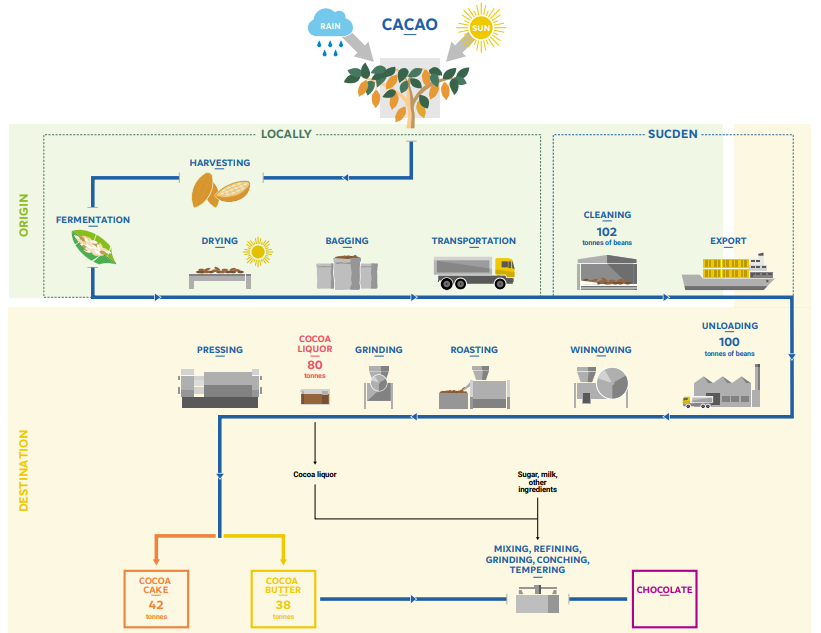
\includegraphics[scale=0.59]{../../Pictures/cacaoprocess.png} 
\label{fig1}
\legend{Fonte: \cite{Sucden}}
\end{center}
\end{figure}

O processamento do cacau é dividido em 11 fases majoritárias \cite{3}, são essas:

\begin{enumerate}
\item Colheita/Limpeza: O cacau é retirado cuidadosamente com uma faca para evitar qualquer injúria, após essa colheita cuidadosa acontece a limpeza do interior do cacau.
\item Fermentação: O processo de fermentação demora entre 36 a 72 horas e é um processo complexo e pouco entendido, mas está sendo desvendado com a tecnologia.
\item Secagem: Após a fermentação é necessário reduzir a humidade do cacau de aproximadamente 55$\%$ para 7,5$\%$, e para isso o cacau é deixado em plataformas de concreto para a secagem.
\item Torrefação: A torrefação varia de empresa para empresa e de região para região, pois está muito ligado ao tipo de saber desejado para aquele chocolate produzido, portanto não há um certo ou errado quando se fala do processo de torrefação.
\item Trituramento: Acontece a tritura desses grãos já separados
\item Descasque: Separação da casca do grão propriamente dito.
\item Refino e conchagem: Com o objetivo também de modificar o cheio e o gosto do chocolate, o processo consiste em colocar pressão sobre o chocoalte com aumento de temperatura para emulsificar e arejar o chocolate.
\item Prensagem de licor: Adiciona-se pressão em um sistema com licor de cacau quente e o output é um bolo de cacau.
\item Moagem: Obtenção do licor propriamente dito a partir da prensagem
\item Manteiga de cacau: Outro material obtido a partir da prensagem.
\item Fabricação do chocolate: Processo de fabricação do chocolate que consiste na temperagem, moldagem, resfriamento e desmoldagem.
\end{enumerate}

\section{Fluxo de produção projetado}

Na maioria das empresa o cacau é recebido em amêndoas após o processo de fermentação e secagem, devido a eficiência e facilidade no transporte desse tipo de carga. Por isso, o processo estudado nesse trabalho irá utilizar esse tipo de matéria-prima, e também diferentemente dos processos majoritários citados acima, a linha de produção usada nesse trabalho não realiza a prensagem, moagem do líquor e nem a obtenção de manteiga de cacau, focando apenas na produção de barras de chocolate de 3 tipos: chocolate amargo 70$\%$, chocolate meio amargo 50$\%$ e chocolate ao leite. Dessa forma o processo segue o seguinte fluxo:

\begin{figure}[H]
\begin{center}
\caption{Fluxograma do processamento de cacau da linha de produção projetada}
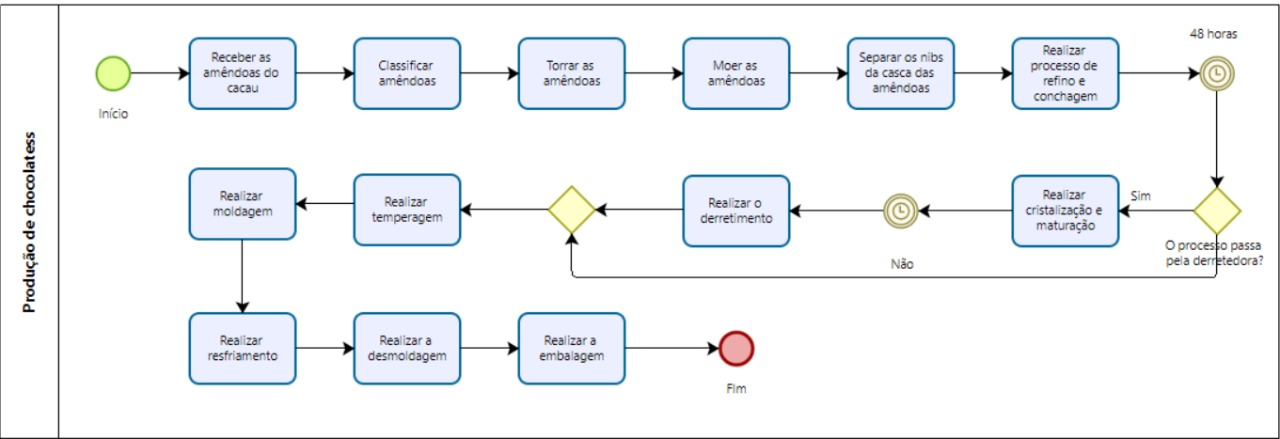
\includegraphics[scale=0.34]{../../Pictures/fluxo1.jpeg} 
\label{figfluxo}
\legend{Fonte: Autoria própria}
\end{center}
\end{figure}

Desse modo, a primeira etapa do processo como já citado é o recebimento das amêndoas, nessa fase ocorre a conferência do produto e sua respectiva nota fiscal e o descarregamento dos sacos de amêndoa do caminhão no estoque primário destinado à matéria-prima. Em seguida é realizada a classificação, essa etapa é de grande importância para que a qualidade dos produtos sempre estejam de acordo com o padrão da empresa, com isso são realizados testes sensoriais e medições de indicadores para destinação correta de cada qualidade de amêndoa.

Após classificadas, as amêndoas seguem para a torrefação que acontece em torradores industriais à 110ºC durante 25 a 30 minutos, por meio dessa atividade as sementes perdem aproximadamente 5$\%$ de água e seus aromas são intensificados. Já torradas, as amêndoas são trituradas em moedores industriais para tornar possível a separação do nibs da casca e facilitar o refino do cacau. Assim, a próxima etapa é realizada é a separação das cascas, nessa parte é utilizado um descascador que retira em torno de 12$\%$ da massa das amêndoas que é referente as cascas. Essas cascas retiradas são descartadas e o processo segue apenas com o nibs do cacau.

\begin{figure}[H]
\begin{center}
\caption{Separação da casca do cacau do nibs}
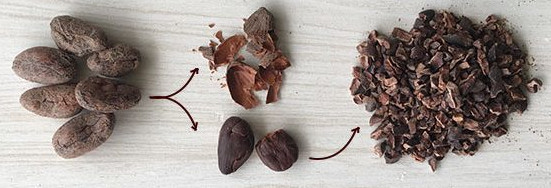
\includegraphics[scale=3]{../../Pictures/nibs1.jpg} 
\label{figtemp}
\legend{Fonte: \cite{nibs}}
\end{center}
\end{figure}

O próximo processo na linha de produção é o refino e conchagem desse nibs do cacau, essas duas atividades são realizadas na máquina melanger (Figura \ref{figmelanger}) e durante a primeira etapa de refino são adicionados os outros ingredientes da receita que a linha está fazendo. No caso da receita de chocolate amargo 70$\%$ é adicionado 30$\%$ de açúcar refinado, na receita de chocolate meio-amargo 50$\%$ são adicionados 15$\%$ de manteiga de cacau e 35$\%$ de açúcar refinado, já o chocolate ao leite possui a adição de 25$\%$ de manteiga de cacau, 25$\%$ de leite em pó integral e 30$\%$ de açúcar refinado. Nas composições dos produtos não há a adição de conservantes e emulsificantes. Essa etapa dura em torno de 48 horas e nela o chocolate é aquecido a uma temperatura de 50ºC e pressionado contra os rolos de pedra da máquina a uma pressão de 4 bar. E a etapa de conchagem, que ocorre em sequência, consiste na manutenção dessas configurações por mais 24 até 48 horas, sem adição de mais nenhum ingrediente. Em conjunto, essas atividades realizam a mistura, agitação, emulsificação e arejamento do chocolate, além de refinar partículas maiores de açúcar e retirar a acidez e o amargor indesejado do produto. \cite{lindt} 

\begin{figure}[H]
\begin{center}
\caption{Máquina melanger em funcionamento}
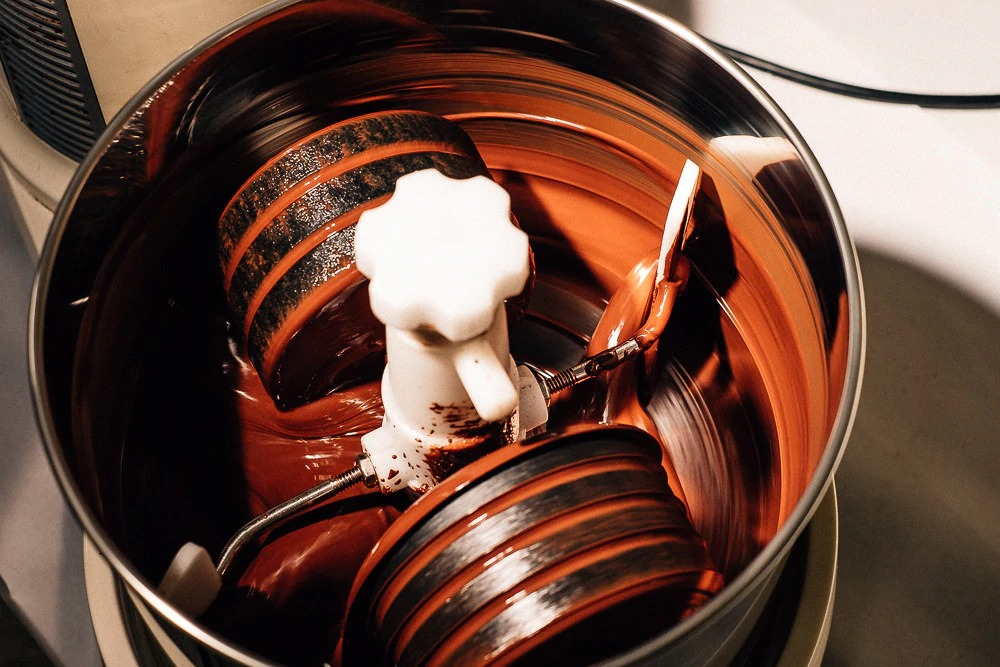
\includegraphics[scale=0.35]{../../Pictures/melanger.jpeg} 
\label{figmelanger}
\legend{Fonte: \cite{melanger}}
\end{center}
\end{figure}

Após a etapa de refino e conchagem existem 3 atividades que são opcionais e serão realizadas na linha de produção apenas para chocolates amargos de edições limitadas. Esses 3 processos são: a cristalização, maturação e derretimento. O chocolate ao sair da máquina melanger já refinado pode seguir diretamente para a temperadeira onde será realizada a temperagem do produto, no entanto em casos especiais é interessante antes de realizar essa atividade reservar o chocolate, a cristalização é um processo natural do produto que ao entrar em contato com a temperatura ambiente se solidifica devido a cristalização da manteiga de cacau presente na mistura. Após essa fase é possível reservar o chocolate em salas com temperatura de até 29ºC para que ele possa maturar durante o período de 2 meses até 1 ano, esse processo intensifica os sabores e traz ao produto um maior equilíbrio no paladar. Por ser tão demorado o processo, apenas parte do que será produzido por mês da linha de produção de chocolate amargo passará por ele. Depois dessa maturação esse chocolate é derretido em temperaturas controladas e passa pela temperadeira assim como os outros.

Na temperadeira ocorre a temperagem do chocolate, que consiste no aumento da temperatura da mistura até 40ºC - 46ºC e o resfriamento lento até 27ºC a 29ºC, a imagem \ref{figtemp} mostra essa variação lenta de temperatura e as fases da temperagem. Por causa disso, o chocolate de entrada deve estar por volta de 32ºC até 35ºC para que possa ocorrer esse aquecimento e também o resfriamento de forma controlada, assim antes de adicionar o chocolate à temperadeira, é necessário reservá-lo durante um curto período após ele sair da melanger ou da derretedeira para que ele possa resfriar, porém sem cristalizar. Esse processo é de extrema importância para a aparência e textura do produto final e também para que o processo de desmolde ocorra sem problemas, nessa etapa os cristais da manteiga de cacau se organizam de maneira mais estável devido o resfriamento lento, e fazem com que o produto final fique crocante à temperatura ambiente (\textit{snap}), tenha brilho e contraia quando esfriado para que consiga se soltar do molde, além de muitas outras características.

\begin{figure}[H]
\begin{center}
\caption{Gráfico da temperatura durante o processo de temperagem}
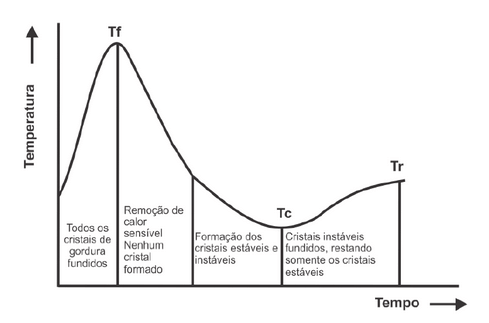
\includegraphics[scale=0.7]{../../Pictures/graficotemperagem.png} 
\label{figtemp}
\legend{Fonte: \cite{temp}}
\end{center}
\end{figure}

Com o chocolate já temperado ocorre o processo de moldagem por meio de uma dosadora e uma mesa vibratória que retira as bolhas de ar de dentro da mistura e esparrama o chocolate por todo o molde. Esse produto então é encaminhado para um túnel de resfriamento para que o chocolate se solidifique de maneira mais rápida e possa ser desmoldado com facilidade que é a etapa seguinte. Após a desmoldagem, que consiste na separação do molde que será limpo e reutilizado posteriormente da barra de chocolate, ocorre por último a embalagem desse chocolate em embalagens primárias, secundárias e terciárias para o transporte final desse produto diretamente para revendedores ou centros de distribuição.

\begin{comment}
Os detalhes de maquinário, temperaturas, tempos de processamento e perdas de cada processo podem ser encontrados na tabela \ref{table6}. As temperaturas com a notação (a) se referem à temperatura ambiente e os tempos de processamento são apenas aproximações feitas de acordo com as capacidades produtivas de algumas máquinas pesquisadas. Além disso, como dito anteriormente os processos de cristalização e maturação ocorrem de maneira natural e não são necessárias máquinas, apenas recipientes e locais adequados para armazenamento.

{\fontsize{7.7}{10}\selectfont
\begin{center}
\begin{longtable}[c]{|
>{\columncolor[HTML]{EFEFEF}}l |c|c|cc|c|}
\caption{Informações de maquinários, temperaturas, tempos e perdas de cada etapa do processo}
\label{table6}\\
\hline
\multicolumn{1}{|c|}{\cellcolor[HTML]{EFEFEF}} &
  \cellcolor[HTML]{EFEFEF} &
  \cellcolor[HTML]{EFEFEF} &
  \multicolumn{2}{c|}{\cellcolor[HTML]{EFEFEF}\textbf{Temperaturas (ºC)}} &
  \cellcolor[HTML]{EFEFEF} \\ \cline{4-5}
\multicolumn{1}{|c|}{\multirow{-2}{*}{\cellcolor[HTML]{EFEFEF}\textbf{Etapas}}} &
  \multirow{-2}{*}{\cellcolor[HTML]{EFEFEF}\textbf{Máquina}} &
  \multirow{-2}{*}{\cellcolor[HTML]{EFEFEF}\textbf{Tempo (h)}} &
  \multicolumn{1}{c|}{\cellcolor[HTML]{EFEFEF}\textbf{Entrada}} &
  \cellcolor[HTML]{EFEFEF}\textbf{Saída} &
  \multirow{-2}{*}{\cellcolor[HTML]{EFEFEF}\textbf{Perdas}} \\ \hline
\endhead
%
\textbf{1. Classificação} &
  - &
  0,20 &
  \multicolumn{1}{c|}{25 - 29 (a)} &
  25 - 29 (a) &
  2\% \\ \hline
\textbf{2. Torrefação} &
  Torrador industrial &
  0,50 &
  \multicolumn{1}{c|}{25 - 29 (a)} &
  110 &
  5\% \\ \hline
\textbf{3. Moagem} &
  Moedor industrial &
  0,20 &
  \multicolumn{1}{c|}{110} &
  25 - 29 (a) &
  2\% \\ \hline
\textbf{4. Descasque} &
  Descascador de amêndoas &
  0,20 &
  \multicolumn{1}{c|}{25 - 29 (a)} &
  25 - 29 (a) &
  12\% \\ \hline
\textbf{5. Refino + Conchagem} &
  Melanger &
  96,00 &
  \multicolumn{1}{c|}{25 - 29 (a)} &
  50 &
  4\% \\ \hline
\textbf{6. Cristalização} &
  - &
  0,50 &
  \multicolumn{1}{c|}{50} &
  25 - 29 (a) &
  1\% \\ \hline
\textbf{7. Maturação} &
  - &
  \multicolumn{1}{l|}{1440,00 - 8760,00} &
  \multicolumn{1}{c|}{25 - 29 (a)} &
  25 - 29 (a) &
  2\% \\ \hline
\textbf{8. Derretimento} &
  Derretedeira de chocolate &
  0,50 &
  \multicolumn{1}{c|}{25 - 29 (a)} &
  42 &
  2\% \\ \hline
\textbf{9. Temperagem} &
  Temperadeira &
  0,35 &
  \multicolumn{1}{c|}{35} &
  28 &
  2\% \\ \hline
\textbf{10. Moldagem} &
  Dosadora + Mesa vibratória &
  0,35 &
  \multicolumn{1}{c|}{28} &
  25 - 29 (a) &
  1\% \\ \hline
\textbf{11. Resfriamento} &
  Túnel de resfriamento &
  0,50 &
  \multicolumn{1}{c|}{25 - 29 (a)} &
  12 &
  0\% \\ \hline
\textbf{12. Desmolde} &
  - &
  0,35 &
  \multicolumn{1}{c|}{12} &
  20 &
  1\% \\ \hline
\textbf{13. Embalagem} &
  Embaladora &
  0,50 &
  \multicolumn{1}{c|}{20} &
  20 &
  1\% \\ \hline
\end{longtable}
\centering \footnotesize{Fonte: Autoria própria}
\end{center}
}

{\fontsize{7}{10}\selectfont
\begin{center}
\begin{longtable}[c]{|
>{\columncolor[HTML]{EFEFEF}}c |c|c|c|c|c|c|}
\caption{Maquinário detalhado}
\label{maquina}\\
\hline
\textbf{Máquina} &
  \cellcolor[HTML]{EFEFEF}\textbf{\begin{tabular}[c]{@{}c@{}}Dimensões\\ (AxLxP) (m)\end{tabular}} &
  \cellcolor[HTML]{EFEFEF}\textbf{\begin{tabular}[c]{@{}c@{}}Potência\\ (kW)\end{tabular}} &
  \cellcolor[HTML]{EFEFEF}\textbf{Capacidade} &
  \cellcolor[HTML]{EFEFEF}\textbf{Material} &
  \cellcolor[HTML]{EFEFEF}\textbf{\begin{tabular}[c]{@{}c@{}}Setup\\ (min)\end{tabular}} &
  \cellcolor[HTML]{EFEFEF}\textbf{Especificações} \\ \hline
\endhead
%
\textbf{Torrador industrial} &
  1,8 x 1,4 x 1,4 &
  8,0 &
  5,0 (kg) &
  - &
  15 &
  - \\ \hline
\textbf{Moedor industrial} &
   &
   &
   &
   &
   &
   \\ \cline{1-1}
\textbf{Descascador de amêndoas} &
  \multirow{-2}{*}{1,3 x 0,8 x 1,3} &
  \multirow{-2}{*}{2,2} &
  \multirow{-2}{*}{10 (kg)} &
  \multirow{-2}{*}{Inox} &
  \multirow{-2}{*}{90} &
  \multirow{-2}{*}{400 kg/h} \\ \hline
\textbf{Melanger*} &
  1,2 x 0,7 x 0,7 &
  0,75 &
  20,0 (kg) &
  \begin{tabular}[c]{@{}c@{}}Inox 304 e \\ Granito Cinza\end{tabular} &
  30 &
  - \\ \hline
\textbf{Compressor de ar} &
  0,3 x 0,6 x 0,6 &
  1,5 &
  25,0 (l) &
  - &
  - &
  - \\ \hline
\textbf{Derretedeira de chocolate} &
  0,7 x 0,6 x 0,4 &
  7,5 &
  50,0 (kg) &
  Inox 304 &
  60 &
  - \\ \hline
\textbf{Temperadeira} &
  0,7 x 0,5 x 0,6 &
  2,9 &
  5,0 (kg) &
  Inox 304 &
  60 &
  5 kg a cada 8min \\ \hline
\textbf{Dosadora (Ø30)} &
  1,5 x 1,1 x 1,4 &
  0,02 &
  40,0 (l) &
  Inox &
  60 &
  \begin{tabular}[c]{@{}c@{}}8 pistões - 50g/pistão\\ 20 ciclos/min\end{tabular} \\ \hline
\textbf{Mesa vibratória*} &
  0,7 x 1,1 x 0,6 &
  0,2 &
  - &
  Inox 304 &
  10 &
  - \\ \hline
\textbf{Túnel de resfriamento} &
  1,2 x 0,6 x 9,0 &
  5,4 &
  - &
  Inox 304 &
  20 &
  - \\ \hline
\textbf{Embaladora} &
  3,3 x 2,9 x 1,4 &
  3,1 &
  - &
  - &
  20 &
  350 pacotes/min \\ \hline
\end{longtable}
*Máquinas que utilizam Compressor de ar \\
\centering \footnotesize{Fonte: Autoria própria}
\end{center}
}
\end{comment}

\section{Resíduos da produção}

Como a indústria de chocolates apresenta resíduos com grande quantidade de matéria
orgânica faz-se necessário um tratamento prévio para seu descarte correto, uma vez que
elevado conteúdo de matéria orgânica pode causar uma diminuição do oxigênio dissolvido
nos rios, com aumento da concentração de microrganismos heterotróficos e,
consequentemente, a elevação da demanda bioquímica de oxigênio. Isso pode gerar uma
modificação da classe do rio, o que é indesejável.

A indústria da alimentação no Brasil e no mundo vem demonstrando claros esforços
para tornar-se mais sustentável. Desde a Conferência Rio-92, o setor tem se engajado nos
debates internacionais sobre desenvolvimento sustentável e se esforçado para desenhar e
adotar as melhores práticas \cite{CNI}.
 
A gestão de resíduos em todo o ciclo de vida de um produto está mudando de patamar
no Brasil com a aprovação da Política Nacional de Resíduos Sólidos. Antes mesmo da
aprovação da Política Nacional de Resíduos, no entanto, as empresas do setor vinham
aplicando tecnologias e políticas para reaproveitar os resíduos dos processos produtivos e as embalagens finais usadas de seus produtos \cite{CNI}.
 
De modo geral, podemos dividir os resíduos da indústria de chocolates em três classes:

\begin{itemize}
\item Efluentes líquidos,
\item Resíduos sólidos,
\item Resíduos pós-consumo.
\end{itemize}

\subsection{Tratamento dos efluentes}

Os efluentes líquidos consistem basicamente por resíduos de limpeza e esgoto
sanitário da empresa em geral. Por ser de pequeno porte, o destino dos efluentes líquidos é a
rede de esgoto pública sem um tratamento prévio específico.
Para ser lançada novamente a bacia hídrica, no entanto, faz-se necessário um
tratamento pela instituição responsável. Nesse caso, como o efluente apresenta origem
industrial torna-se indispensável um tratamento biológico devido às altas concentrações de
matéria orgânica e nutrientes.

O tratamento biológico de resíduos emprega a ação conjunta de espécies diferentes de
microrganismos em biorreatores, que operados sob determinadas condições resulta na
estabilização dos mesmos. Em geral, os diferentes tipos de microrganismos nos processos
biológicos de tratamento atuam conjuntamente, formando uma verdadeira cadeia alimentar
com interações nutricionais facultativas e obrigatórias.

\subsection{Tratamento dos resíduos sólidos}

Os resíduos sólidos da indústria se dividem basicamente em produtos que serão
reprocessados, dejetos destinados aos aterros sanitários e de resíduos sólidos industriais e
materiais para reciclagem.

Em situações onde variáveis de processo estão fora de controle ou há a quebra da barra
antes da distribuição duas medidas podem ser tomadas: ou ocorre o reprocesso da massa de
chocolate, adicionando-se no máximo à razão de 10$\%$ do chocolate reprocessado sobre o
produto em linha; ou ainda o destino final da massa torna-se a venda para fabricação de
chocolate granulado e coberturas.

Os resíduos sólidos dos setores distintos da área produtiva são enviados para aterros
sanitários, por se tratarem de resíduos não perigosos segundo a classificação da norma
10004/2004 da ABNT \cite{ABNT}. Esses aterros são utilizados para a disposição de
resíduos sólidos urbanos no solo, sem causar danos à saúde pública e ao meio ambiente,
minimizando os impactos ambientais. Nesse caso, os resíduos são confinados na menor área
possível, reduzindo-os ao menor volume permissível, cobrindo-os com uma cama de terra
quando necessário. Esse método deve conter todos os elementos de proteção ambiental
\cite{FEAM}.

De acordo com a Resolução CONAMA n° 313/2002, o resíduo sólido industrial é todo
resíduo que resulte de atividades industriais e que se encontre nos estados sólido, semi sólido,
gasoso – quando contido, e líquido – cujas particularidades tornem inviável o seu lançamento
na rede pública de esgoto ou em corpos d’água, ou exijam para isso soluções técnicas ou
economicamente inviáveis em face da melhor tecnologia disponível \cite{PNRS}. Assim, os
resíduos sólidos da área produtiva são encaminhados para empresas terceirizadas que realizam
o descarte adequado.

Os materiais e embalagens danificadas que podem ser reciclados são separados e
recolhidos por empresas terceirizadas, sendo enviados para a reciclagem. Isso ocorre porque a
reciclagem de resíduos sólidos é uma alternativa viável para propiciar à preservação de
recursos naturais, a economia de energia, a redução da área que demanda o aterro sanitário, a
geração de emprego e renda, assim como a conscientização da população para questões
ambientais \cite{Ole}.

\subsection{Tratamento dos resíduos pós-consumo}

Existe uma preocupação em garantir um destino para as embalagens dos chocolates
em barra após o consumo. Para isso, ocorre a reciclagem do material polimérico, onde a
estrutura do material residual é alterada, de modo que os subprodutos resultantes possam ser
usados para outros fins que não a produção do material original, uma vez que em indústria de
alimentos não se pode utilizar materiais reciclados \cite{oliveira}.





\newpage
\chapter{Balanço de Massa}
%\pagestyle{fancy}

O balanço de massa é crucial para a análise de um novo processo, bem como um já existente. Esse cálculo consiste em uma igualdade entre toda a massa que entra no sistema e a massa que sai, como mostrado na equação \ref{eq1}, onde \textit{e$_{i}$} são as entradas de massa no sistema e \textit{s$_{j}$} são as saídas. 

\begin{equation}
\sum\limits_{i=1}^{n}e_{i}=\sum\limits_{j=1}^{n}s_{j}
\label{eq1}
\end{equation}

O entendimento do processo de produção é fundamental para o dimensionamento desses materiais que entram no sistema, e também para quantificar as perdas que acontecem em cada etapa. Assim, foi criado um fluxograma mais completo que abrange também as saídas e entradas de materiais em cada fase.

\begin{figure}[H]
\begin{center}
\caption{Fluxograma para Balanço de Massa}
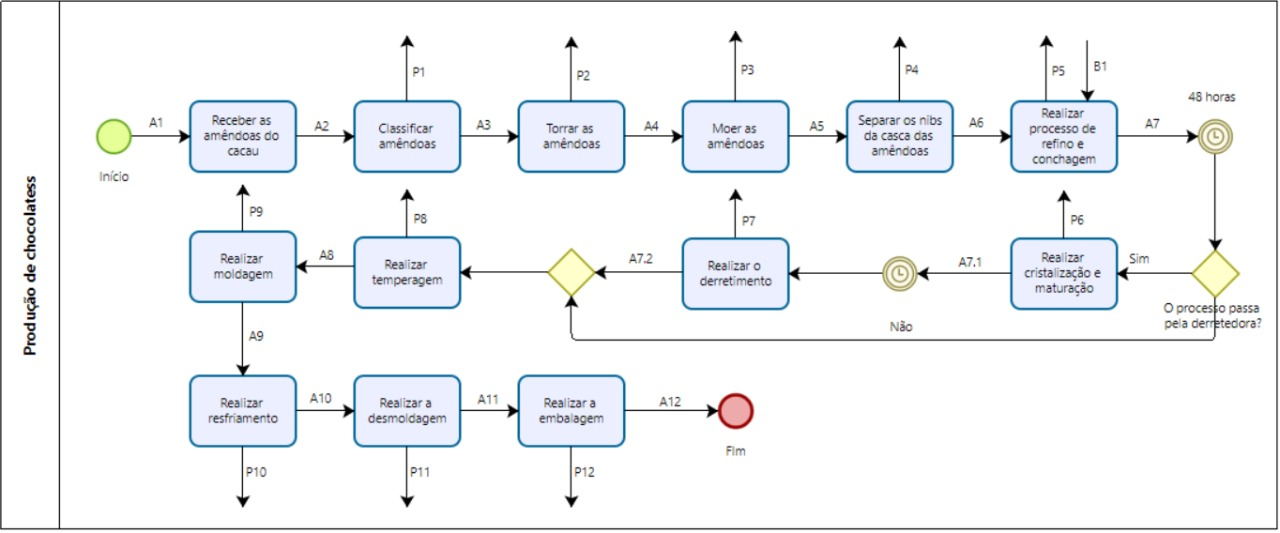
\includegraphics[scale=0.34]{../../Pictures/fluxo2.jpeg} 
\label{fluxo2}
\legend{Fonte: Autoria Própria}
\end{center}
\end{figure}

Parte das perdas de massa que ocorrem são planejadas. Essas perdas consistem na retirada da água das amêndoas, na etapa de torrefação, e na separação da casca que ocorre após o processo de moagem. E o restante das perdas ocorrem devido a falhas no processo produtivo, muitas vezes falhas humanas ou limitações das próprias máquinas que impossibilitam o aproveitamento completo de todo o material que é passado por ela. Essas perdas foram estimadas entre 1$\%$ e 4$\%$, dependendo da complexidade da máquina e da interferência humana no processo. 

Além disso, no fluxograma da imagem \ref{fluxo2}, o valor de B1 varia conforme a receita que está sendo feita na linha de produção. Para a receita de chocolate amargo esse valor corresponde apenas ao açúcar que é adicionado, enquanto na receita de chocolate meio amargo o B1 representa a solução de açúcar e manteiga de cacau que é adicionada. E por fim, na receita de chocolate ao leite esse valor corresponde a uma mistura de açúcar, leite e manteiga de cacau.

Nas figuras a seguir se encontram os balanços de massa das 3 receitas produzidas na linha, todas utilizaram como base uma entrada de 100kg de amêndoas de cacau (Entrada 1). A imagem \ref{bm1} se baseia na receita de 70$\%$ líquor de cacau 30$\%$ açúcar, a imagem \ref{bm2} utiliza como base a receita de 50$\%$ líquor de cacau, 35$\%$ açúcar e 15$\%$ manteiga de cacau, e a imagem \ref{bm3} representa a receita de chocolate ao leite composta por 20$\%$ líquor de cacau, 25$\%$ manteiga de cacau, 25$\%$ leite integral e 30$\%$ açúcar. Nas tabelas, a Entrada 2 representa o açúcar, a Entrada 3 a manteiga de cacau e a Entrada 4 o leite integral, a perda e a saída foram calculados em quilogramas (kg).


\begin{figure}[H]
\begin{center}
\caption{Balanço de Massa - Chocolate Amargo 70\%}
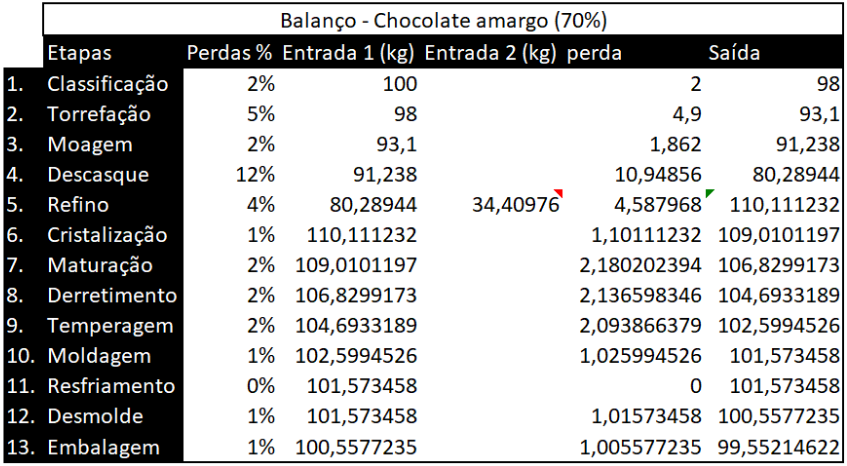
\includegraphics[scale=0.46]{../../Pictures/bm1.png} 
\label{bm1}
\legend{Fonte: Autoria Própria}
\end{center}
\end{figure}

\begin{figure}[H]
\begin{center}
\caption{Balanço de Massa - Chocolate Meio Amargo 50\%}
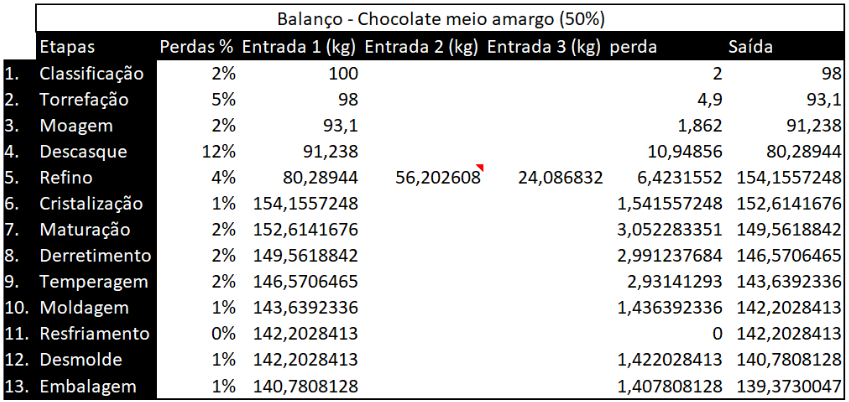
\includegraphics[scale=0.53]{../../Pictures/bm2.png} 
\label{bm2}
\legend{Fonte: Autoria Própria}
\end{center}
\end{figure}

\begin{figure}[H]
\begin{center}
\caption{Balanço de Massa - Chocolate ao Leite}
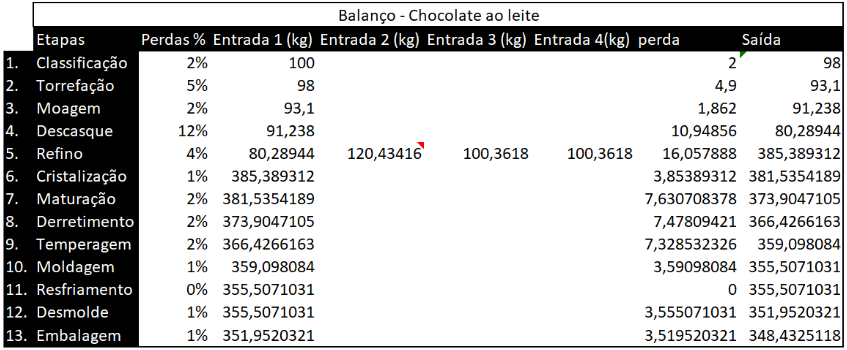
\includegraphics[scale=0.53]{../../Pictures/bm3.png} 
\label{bm3}
\legend{Fonte: Autoria Própria}
\end{center}
\end{figure}

\newpage
\chapter{Balanço de Energia}
%\pagestyle{fancy}

O Balanço de energia é essencial para a estruturação e mapeamento de rotas produtivas. Para a realização do balanço de energia do sistema consideramos a 1ª lei da Termodinâmica, ou seja, a energia total transferida para o sistema é a variação de suas energias internas. Dessa forma, seguindo o fluxograma do processo e considerando as perdas calculadas no balanço de massa, foi realizado o balanço de energia do sistema e produção de chocolate para os três tipos de produtos finais (chocolate amargo, meio amargo e ao leite).

Tanto o balanço de massa quanto o balanço de energia possuem fundamental relevância em um processo industrial, ambos garantem uma segurança em relação ao mapeamento e estrutura de todo o projeto, além de compilar dados essenciais para averiguação de alterações nos resultados da produção.  Além de constar um embasamento teórico e técnico da rota de produção. 

Energia é a capacidade de um sistema de realizar trabalho ou gerar calor, e ela pode ser transferida em um sistema aberto ou fechado. Todos os processos industriais estão associados a alterações energéticas sob as mais variadas formas:

\begin{itemize}
\item Processo com reação química: (endotérmico e exotérmico).
\item Processo de combustão: energia interna do combustível é utilizada para geração de calor (fornos, caldeiras), ou para produção de trabalho (motores e turbinas).
\item Bombas e Compressores: fornece trabalho para acelerar ou comprimir fluidos.
\item Trocadores de Calor: transfere-se calor de um fluido quente para um fluido frio.
\end{itemize}

A produção de chocolate através do cacau consiste em 13 etapas de processos industriais. Dentre eles os processos de: torrefação, moagem, refino cristalização, derretimento, temperagem, resfriamento e desmolde; apresentam trocas de energia.
 
No sistema analisado foram identificadas alterações energéticas através de compressores (refrigerador usado no processo de resfriamento) e trocadores de calor nos processos de torrefação (troca de calor e perda de umidade da amêndoa e o torrador), moagem (resfriamento da amêndoa na transição de um processo para outro), refino (aumento da temperatura dos ingredientes em temperatura ambiente até 50°C), cristalização (resfriamento da amêndoa na transição de um processo para outro), derretimento (aumento da temperatura do chocolate e derretimento), temperagem (resfriamento do chocolate com a troca com o ambiente) e por fim nos processos de resfriamento (diminuição da temperatura do chocolate e trabalho realizado pelo compressor do refrigerador) e desmolde (troca de calor com o ambiente na transição de um processo para outro). Processos de reação química com o derretimento da sacarose foram desconsiderados para esse estudo.

As tabelas abaixo mostram os valores encontrados para o balanço de energia dos três tipos de chocolates, considerando a entrada de 1kg de amêndoa no início do processos e todos os valores de energia em kcal/kg.

\begin{figure}[H]
\begin{center}
\caption{Balanço de Energia - Chocolate Amargo}
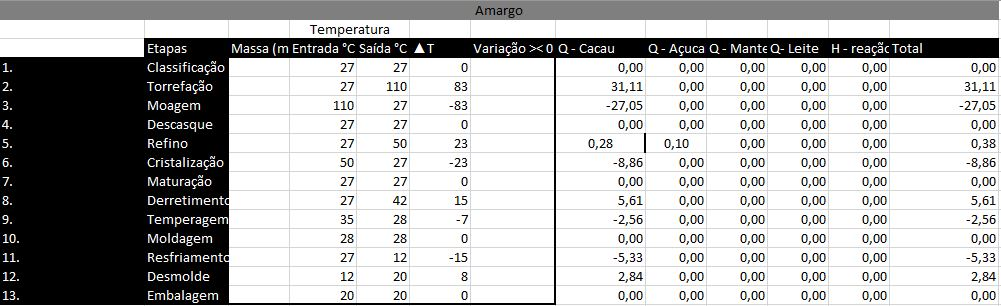
\includegraphics[scale=0.5]{../../Pictures/amargo.jpg} 
\legend{Fonte: Autoria Própria}
\end{center}
\end{figure}

\begin{figure}[H]
\begin{center}
\caption{Balanço de Energia - Chocolate Meio Amargo}
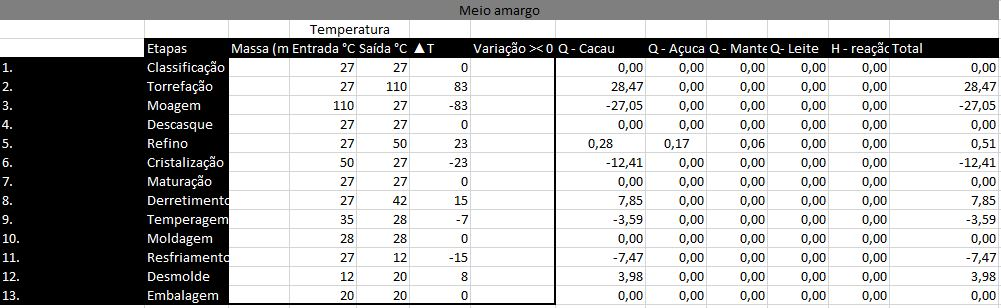
\includegraphics[scale=0.5]{../../Pictures/meio amargo.jpg} 
\legend{Fonte: Autoria Própria}
\end{center}
\end{figure}

\begin{figure}[H]
\begin{center}
\caption{Balanço de Energia - Chocolate Ao Leite}
\includegraphics[scale=0.5]{../../Pictures/ao leite.jpg} 
\legend{Fonte: Autoria Própria}
\end{center}
\end{figure}


Além dos cálculos realizados com as diferenças de temperatura de cada estágio, foram realizados os cálculos de energia consumida no túnel de resfriamento, pois nele ocorre a retirada de energia do chocolate por meio da troca de calor com uma solução de amõnia no equipamento de forma indireta. Dessa forma foi possível verificar se o equipamento possuia capacidade suficiente para realizar o resfriamento e dimensionar de forma muito mais precisa o gasto energético.

Para esses cálculos foram utilizadas: a tabela de propriedades na saturação e o diagrama de p-h da amônia, que se encontram nos Anexos A e B, respectivamente. Nos cálculos foram estipulados os valores de 0°C no evaporador e 40°C na saída do condensador para a solução de amônia e uma eficiência de 75$\%$.

\begin{figure}[H]
\begin{center}
\caption{Fluxograma de um refrigerador}
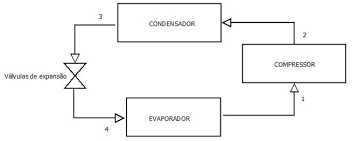
\includegraphics[scale=1]{../../Pictures/esquema.png} 
\legend{Fonte: Autoria Própria}
\end{center}
\end{figure}

Dessa forma, foi possível verificar que o túnel de resfriamento consome 33,13 kcal para resfriar 1 kg de chocolate, independente do tipo. Como a empresa está dimensionada para produzir por volta de 115 kg/h de chocolate, a energia consumida no túnel de resfriamento gira em torno de 3827,17 kcal/h, ou seja, 4,45 kW. Portanto, foi possível verificar que o túnel de resfriamento consegue suprir toda a demanda da fábrica e que o consumo de energia é um pouco abaixo da potência máxima do equipamento.



\newpage
\chapter{Oferta e Demanda}

As pesquisas realizadas sobre consumo aparente de chocolate no Brasil não são suficientes para realizar uma projeção válida para os próximos dez anos, já que não foi possível encontrar dados consistentes sobre a produção, exportação e importação de chocolate em barras no Brasil nos últimos dez anos.

Segundo as últimas pesquisas, o modo como o chocolate é consumido no Brasil está mudando. Os brasileiros consomem menos em quantidade, porém gastam mais, isso se reflete no aumento do faturamento das empresas do setor nos últimos anos e também em uma pequena queda no consumo interno em toneladas. Logo, o mercado de chocolates finos vem crescendo, porém o mercado como um todo não está expandindo. Portanto, a Showcolate! busca se inserir nessa parcela de crescimento do mercado de chocolates finos, com uma boa estratégia de marketing e muita qualidade a empresa busca uma fatia de mercado de 3$\%$ do crescimento do mercado de chocolates premium/finos, esse valor corresponde a aproximadamente 0,02$\%$ de todo o mercado de chocolate.

Dessa forma foi tomado como base o consumo aparente de chocolates no ano de 2021, correspondente a 679 mil toneladas. Tendo em vista que de acordo com dados divulgados o setor de chocolates finos representa 7$\%$ do total de chocolates consumidos e que o crescimento anual aproximado do mercado de chocolates no Brasil é de 10$\%$, esses números foram tomados como base para prever o crescimento do setor. \cite{c2-1} \cite{c2-2} \cite{4}

Dentro do crescimento esperado foi projetado a participação de 3$\%$ de fatia desse mercado para a empresa ShowColate!. Assim a equação que descreve ficou da seguinte forma.

Para o ano zero (no nosso caso = 2023):

Demanda (ton) = 679.000*0,07*(0,1*0,03)

E para os anos seguintes:

Demanda (ton) = Demanda (n-1) *1,1

Desse modo foi possível calcular a demanda prevista para os próximos anos seguindo as previsões de um crescimento de 10$\%$ ao ano do mercado de chocolates premium/finos.

\begin{figure}[H]
\begin{center}
\caption{Demanda prevista}
\includegraphics[scale=0.5]{../../../../../../Downloads/WhatsApp Image 2022-09-02 at 19.02.32.jpeg} 
\legend{Fonte: Autoria própria}
\end{center}
\end{figure}

E para dimensionamento da indústria foi definida como meta para a capacidade efetiva a da previsão de demanda de 2030, ou seja, próximo a 250 toneladas por ano. Desse modo, foi preciso realizar cálculos para definição de capacidade de cada máquina, tempo de setup e eficiência. Os setups, principalmente os focados em limpeza foram deduzidos como frequentes, ocorrendo em muitas máquinas diariamente, e a eficiência foi estabelecida como 95$\%$. Já a capacidade foi analisada de acordo com o tempo de processamento e o dimensionamento do maquinário. 

{\fontsize{7}{10}\selectfont
\begin{center}
\begin{longtable}[c]{|
>{\columncolor[HTML]{EFEFEF}}c |c|c|c|c|c|c|}
\caption{Maquinário detalhado}
\label{maquina}\\
\hline
\textbf{Máquina} &
  \cellcolor[HTML]{EFEFEF}\textbf{\begin{tabular}[c]{@{}c@{}}Dimensões\\ (AxLxP) (m)\end{tabular}} &
  \cellcolor[HTML]{EFEFEF}\textbf{\begin{tabular}[c]{@{}c@{}}Potência\\ (kW)\end{tabular}} &
  \cellcolor[HTML]{EFEFEF}\textbf{Capacidade} &
  \cellcolor[HTML]{EFEFEF}\textbf{Material} &
  \cellcolor[HTML]{EFEFEF}\textbf{\begin{tabular}[c]{@{}c@{}}Setup\\ (min)\end{tabular}} &
  \cellcolor[HTML]{EFEFEF}\textbf{Especificações} \\ \hline
\endhead
%
\textbf{Torrador industrial} &
  1,8 x 1,4 x 1,4 &
  8,0 &
  20,0 (kg) &
  - &
  15 &
  - \\ \hline
\textbf{Moedor industrial} &
   &
   &
   &
   &
   &
   \\ \cline{1-1}
\textbf{Descascador de amêndoas} &
  \multirow{-2}{*}{1,3 x 0,8 x 1,3} &
  \multirow{-2}{*}{2,2} &
  \multirow{-2}{*}{30,0 (kg)} &
  \multirow{-2}{*}{Inox} &
  \multirow{-2}{*}{90} &
  \multirow{-2}{*}{400 kg/h} \\ \hline
\textbf{Melanger*} &
  1,2 x 0,7 x 0,7 &
  0,75 &
  100,0 (kg) &
  \begin{tabular}[c]{@{}c@{}}Inox 304 e \\ Granito Cinza\end{tabular} &
  30 &
  - \\ \hline
\textbf{Compressor de ar} &
  0,3 x 0,6 x 0,6 &
  1,5 &
  25,0 (l) &
  - &
  - &
  - \\ \hline
\textbf{Derretedeira de chocolate} &
  0,7 x 0,6 x 0,4 &
  7,5 &
  50,0 (kg) &
  Inox 304 &
  60 &
  - \\ \hline
\textbf{Temperadeira} &
  0,7 x 0,5 x 0,6 &
  2,9 &
  10,0 (kg) &
  Inox 304 &
  60 &
  5 kg a cada 8min \\ \hline
\textbf{Dosadora (Ø30)} &
  1,5 x 1,1 x 1,4 &
  0,02 &
  40,0 (l) &
  Inox &
  60 &
  \begin{tabular}[c]{@{}c@{}}8 pistões - 50g/pistão\\ 20 ciclos/min\end{tabular} \\ \hline
\textbf{Mesa vibratória*} &
  0,7 x 1,1 x 0,6 &
  0,2 &
  - &
  Inox 304 &
  10 &
  - \\ \hline
\textbf{Túnel de resfriamento} &
  1,2 x 0,6 x 9,0 &
  5,4 &
  100,0 (kg) &
  Inox 304 &
  20 &
  - \\ \hline
\textbf{Embaladora} &
  3,3 x 2,9 x 1,4 &
  3,1 &
  100,0 (kg) &
  - &
  20 &
  350 pacotes/min \\ \hline
\end{longtable}
*Máquinas que utilizam Compressor de ar \\
\centering \footnotesize{Fonte: Autoria própria}
\end{center}
}

\begin{figure}[H]
\begin{center}
\caption{Número de máquinas e produção delas por hora}
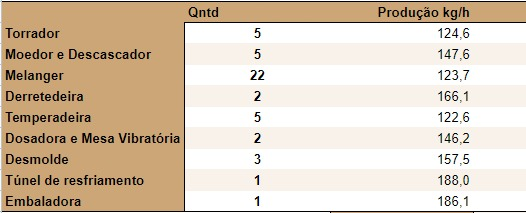
\includegraphics[scale=0.5]{../../Pictures/WhatsApp Image 2022-09-22 at 20.48.19.jpeg} 
\legend{Fonte: Autoria própria}
\end{center}
\end{figure}

Com esses dados calculados e definidos, foi possível chegar em uma capacidade efetiva de 258,9 toneladas por ano. E com os valores representados no gráfico anteriormente com esse valor de capacidade calculado é possível verificar o grau de utilização da indústria da Showcolate!.


% Please add the following required packages to your document preamble:
% \usepackage[table,xcdraw]{xcolor}
% If you use beamer only pass "xcolor=table" option, i.e. \documentclass[xcolor=table]{beamer}
\begin{table}[H]
\centering
\caption{Grau de utilização}
\label{grau}
\begin{tabular}{l|l|l}
\rowcolor[HTML]{EFEFEF} 
\multicolumn{1}{c|}{\cellcolor[HTML]{EFEFEF}\textbf{Ano}} & \multicolumn{1}{c|}{\cellcolor[HTML]{EFEFEF}\textbf{Demanda prevista}} & \multicolumn{1}{c}{\cellcolor[HTML]{EFEFEF}\textbf{Grau de utilização}} \\ \hline
2023                                                      & 0                                                                      & 0\%                                                                     \\ \hline
2024                                                      & 142,6                                                                  & 55\%                                                                    \\ \hline
2025                                                      & 156,8                                                                  & 61\%                                                                    \\ \hline
2026                                                      & 172,5                                                                  & 67\%                                                                    \\ \hline
2027                                                      & 189,8                                                                  & 73\%                                                                    \\ \hline
2028                                                      & 208,8                                                                  & 81\%                                                                    \\ \hline
2029                                                      & 229,6                                                                  & 89\%                                                                    \\ \hline
2030                                                      & 252,6                                                                  & 98\%                                                                   
\end{tabular}
\end{table}


Com esses valores, é possível concluir que será possível suprir a demanda a partir da capacidade produtiva efetiva da fábrica até o ano de 2030, sendo um valor de 250 mil toneladas de chocolate produzido neste ano para igualar à demanda projetada.


Para a implementação da empresa foi considerado o período de um ano. Considerando a necessidade de locação de um espaço apropriado, adequação da fábrica e compra de maquinários, processos legais e especificações técnicas. Além de todos os certificados e inspeções necessárias para atender os requisitos de uma fábrica de produtos alimentícios.

Levando em conta todos esses aspectos foi definido que o período de um ano é necessário para a implementação da fábrica e o início das operações efetivamente a partir do ano de 2024.


\newpage
\chapter{Estudo do Processo Produtivo}

De acordo com os cálculos e previsões feitas para a demanda de chocolate, a fábrica foi projetada para produzir por volta de 142 toneladas no ano de 2024 e chegar ao seu máximo de utilização em 2030, onde produzirá mais de 252 toneladas de chocolate. Dessa quantia está definida a fabricação de 50$\%$ de chocolate amargo 70$\%$, 25$\%$ de chocolate meio amargo, 20$\%$ de chocolate ao leite e 5$\%$ de chocolate amargo 70$\%$ maturado.

\begin{figure}[H]
\begin{center}
\caption{Produção da fábrica por ano}
\includegraphics[scale=0.8]{../../../../../../Downloads/1.jpeg} 
\legend{Fonte: Autoria própria}
\end{center}
\end{figure}

Para a fábrica iniciar com custos menores foi definido apenas 1 turno de trabalho de 8h e 22 dias trabalhados no mês. Essa estratégia vai ao encontro da ideia de uma inserção com cautela no mercado, porém com margem para expansão.

Além disso, foram definidas as escalas de produção para maior eficiência do tempo de setup. As escalas se repetem a cada 2 meses e foram definidas da seguinte forma:

\begin{itemize}
\item dia 1: Chocolate 70$\%$ maturado
\item dia 2 até dia 12: Chocolate 70$\%$
\item dia 13 até dia 17: Chocolate meio amargo
\item dia 18 até dia 26: Chocolate ao leite
\item dia 27 até dia 32: Chocolate meio amargo
\item dia 33 até dia 43: Chocolate 70%
\item dia 44: Chocolate 70$\%$ maturado
\end{itemize}

E por fim, foi definida uma eficiência de 95$\%$ que auxiliou na definição da capacidade produtiva.

\begin{figure}[H]
\begin{center}
\caption{Quantidade de máquinas e especificações}
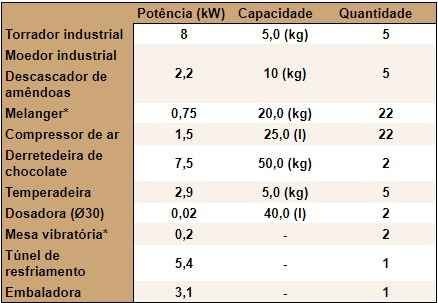
\includegraphics[scale=0.8]{../../Pictures/WhatsApp Image 2022-09-22 at 20.50.16.jpeg} 
\legend{Fonte: Autoria própria}
\end{center}
\end{figure}

Para o cálculo correto de todas as entradas, foi necessário considerar a demanda final de cada um dos produtos, a quantidade de produtos, o percentual de matéria prima demandada para cada um dos 3 produtos finais, além de considerar todas as perdas referentes ao processamento do chocolate. Para isso, realizou-se a iteração de quantidade de entradas necessárias para que fosse possível atingir a demanda de cada um dos produtos.

\begin{figure}[H]
\begin{center}
\caption{Total de insumos necessários em toneladas no ano de 2024}
\includegraphics[scale=0.8]{../../../../../../Downloads/2.jpeg} 
\legend{Fonte: Autoria própria}
\end{center}
\end{figure}

Além disso, era necessário o cálculo do gasto de kw/h de cada uma das máquinas, para assim melhor prever futuramente tanto o custo dos produtos quanto o gasto energético. A tabela a seguir mostra esse gasto energético por cada máquina da fábrica de chocolates.

\begin{figure}[H]
\begin{center}
\caption{Potência do maquinário}
\includegraphics[scale=0.8]{../../../../../../Downloads/3.jpeg} 
\legend{Fonte: Autoria própria}
\end{center}
\end{figure}

Para a produção de cada um dos produtos da cartela da showcolate, foi feito um cálculo a partir da demanda prevista para o ano de início das operações. Além disso, foi considerado o balanço de massa de cada um dos produtos, ou seja, era necessário um $\%$ de matéria prima diferente para cada um dos nossos produtos, e assim foi possível chegar nos dados finais de quantidade produzida em toneladas, como demonstrado na tabela:

\begin{figure}[H]
\begin{center}
\caption{Quantidade produzida em toneladas no ano de 2024}
\includegraphics[scale=0.8]{../../../../../../Downloads/4.jpeg} 
\legend{Fonte: Autoria própria}
\end{center}
\end{figure}


\newpage
\chapter{Localização}
%\pagestyle{fancy}

A definição de um ponto específico para a operação se encontrar é uma decisão de extrema importância para qualquer negócio ou empresa, uma vez que pode definir o sucesso ou insucesso da empresa por diversos fatores. Por isso, para o desenvolvimento deste estudo foram utilizados métodos quantitativos e qualitativos para este fim.

Os dois métodos utilizado foram:

\begin{enumerate}
\item Método dos momentos;
\item Método da ponderação qualitativa.
\end{enumerate}

Tais métodos foram utilizados estrategicamente pela complementaridade entre os dois, o primeiro exigia uma análise mais quantitativa utilizando coordenadas e localizações precisas ou pouco aproximadas, já o  segundo se refere a uma análise mais quantitativa, colocando peses relativos para as localidades segundo critérios pré-acordados e que fazem sentido para o tipo de nicho especificado.

\section{Método dos momentos}

Para o primeiro estudo, foram segmentadas as localizações dos principais fornecedores, adquirindo os seguintes resultados:

\begin{figure}[H]
\begin{center}
\caption{Localizações}
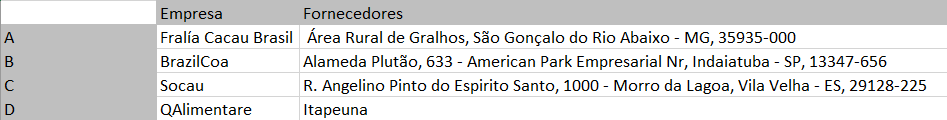
\includegraphics[scale=0.5]{../../Pictures/tabela1.png} 
\label{loca}
\legend{Fonte: Autoria própria}
\end{center}
\end{figure}

Com a definição dessas localidades geográficas, foi possível encontrar as distâncias em km entre as cidades, sendo as seguintes:

\begin{itemize}
\item AB 703km  
\item AD 932km
\item AC 449km
\item BC 1018km
\item BD 343km
\item CD 1179km
\end{itemize}

A partir desses dados, torna-se possível então realizar o cálculo do momento. É importante lembrar que o menor momento é aquele que deve ser escolhido, por representar a melhor localização possível dentre as segmentadas.

\begin{figure}[H]
\begin{center}
\caption{Momentos das localizações}
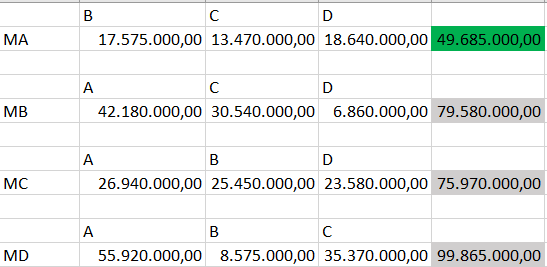
\includegraphics[scale=0.6]{../../Pictures/tabela3.png} 
\label{loca}
\legend{Fonte: Autoria própria}
\end{center}
\end{figure}

Para realizar o cálculo dos momentos é necessário saber o custo do transporte/km, a distância entre as duas cidades.
	
Portanto, com os resultados obtidos é possível concluir que a melhor localização segundo o primeiro método é a localização A: 

\begin{center}
\textbf{Fralía Cacau Brasil | Área Rural de Gralhos, São Gonçalo do Rio Abaixo - MG, 35935-000}
\end{center}

\section{Método da ponderação qualitativa}

Já no segundo método, os cálculos tem uma base qualitativa, ou seja, por meio do conhecimento dos envolvidos, são elencados pesos para os critérios levantados e a partir disso é feito o cálculo da melhor localidade. Os critérios levantados foram os seguintes:

\begin{itemize}
\item Custo do local;
\item Impostos locais;
\item Disponibilidade de MO;
\item Acesso à auto-estradas;
\item Potencial de expansão.
\end{itemize}

Esses critérios levantados foram validados com especialistas na área, portanto confirmou-se a autenticidade e a veracidade da importância desses mesmos.
	
O próximo passo para o método é elencar pesos para cada localidade seguindo cada critério, e o resultado foi o seguinte:

\begin{longtable}[c]{|
>{\columncolor[HTML]{D9D9D9}}c |c|cc|cc|cc|}
\caption{Critérios e notas }
\label{tabela 5}\\
\hline
Critérios &
  \cellcolor[HTML]{D9D9D9}Peso - Relativo &
  \multicolumn{2}{c|}{\cellcolor[HTML]{D9D9D9}São Paulo} &
  \multicolumn{2}{c|}{\cellcolor[HTML]{D9D9D9}Espirito Santo} &
  \multicolumn{2}{c|}{\cellcolor[HTML]{D9D9D9}Minas gerais} \\ \hline
\endhead
%
Custo do local         & 50 & \multicolumn{1}{c|}{2} & 100 & \multicolumn{1}{c|}{3} & 150 & \multicolumn{1}{c|}{4} & 200 \\ \hline
Impostos locais        & 40 & \multicolumn{1}{c|}{4} & 160 & \multicolumn{1}{c|}{3} & 120 & \multicolumn{1}{c|}{3} & 120 \\ \hline
Disponibilidade de MO  & 40 & \multicolumn{1}{c|}{5} & 200 & \multicolumn{1}{c|}{2} & 80  & \multicolumn{1}{c|}{3} & 120 \\ \hline
Acesso à auto-estradas & 10 & \multicolumn{1}{c|}{5} & 50  & \multicolumn{1}{c|}{3} & 30  & \multicolumn{1}{c|}{2} & 20  \\ \hline
Potencial de expansão  & 20 & \multicolumn{1}{c|}{2} & 40  & \multicolumn{1}{c|}{4} & 80  & \multicolumn{1}{c|}{4} & 80  \\ \hline
\end{longtable}

O resultado é a soma da segunda coluna de cada localidade, sendo o seguinte:

\begin{longtable}[c]{cccc|cc|cc|}
\caption{Critérios e notas compilados}
\label{tabela 5}\\
\hline
\rowcolor[HTML]{D9D9D9} 
\multicolumn{1}{|c|}{\cellcolor[HTML]{D9D9D9}Critérios} &
  \multicolumn{1}{c|}{\cellcolor[HTML]{D9D9D9}Peso - Relativo} &
  \multicolumn{2}{c|}{\cellcolor[HTML]{D9D9D9}São Paulo} &
  \multicolumn{2}{c|}{\cellcolor[HTML]{D9D9D9}Espirito Santo} &
  \multicolumn{2}{c|}{\cellcolor[HTML]{D9D9D9}Minas gerais} \\ \hline
\endhead
%
\multicolumn{1}{|c|}{\cellcolor[HTML]{D9D9D9}Custo do local} &
  \multicolumn{1}{c|}{50} &
  \multicolumn{1}{c|}{2} &
  100 &
  \multicolumn{1}{c|}{3} &
  150 &
  \multicolumn{1}{c|}{4} &
  200 \\ \hline
\multicolumn{1}{|c|}{\cellcolor[HTML]{D9D9D9}Impostos locais} &
  \multicolumn{1}{c|}{40} &
  \multicolumn{1}{c|}{4} &
  160 &
  \multicolumn{1}{c|}{3} &
  120 &
  \multicolumn{1}{c|}{3} &
  120 \\ \hline
\multicolumn{1}{|c|}{\cellcolor[HTML]{D9D9D9}Disponibilidade de MO} &
  \multicolumn{1}{c|}{40} &
  \multicolumn{1}{c|}{5} &
  200 &
  \multicolumn{1}{c|}{2} &
  80 &
  \multicolumn{1}{c|}{3} &
  120 \\ \hline
\multicolumn{1}{|c|}{\cellcolor[HTML]{D9D9D9}Acesso à auto-estradas} &
  \multicolumn{1}{c|}{10} &
  \multicolumn{1}{c|}{5} &
  50 &
  \multicolumn{1}{c|}{3} &
  30 &
  \multicolumn{1}{c|}{2} &
  20 \\ \hline
\multicolumn{1}{|c|}{\cellcolor[HTML]{D9D9D9}Potencial de expansão} &
  \multicolumn{1}{c|}{20} &
  \multicolumn{1}{c|}{2} &
  40 &
  \multicolumn{1}{c|}{4} &
  80 &
  \multicolumn{1}{c|}{4} &
  80 \\ \hline
\multicolumn{1}{l}{} &
  \multicolumn{1}{l}{} &
  \multicolumn{1}{l|}{} &
  \cellcolor[HTML]{A0D9AF}550 &
  \multicolumn{1}{l|}{} &
  \cellcolor[HTML]{EFEFEF}460 &
  \multicolumn{1}{l|}{} &
  \cellcolor[HTML]{EFEFEF}540 \\ \cline{4-4} \cline{6-6} \cline{8-8} 
\end{longtable}

Portanto, a partir dos dados acima é possível concluir que os dois melhores estados para se definir a localização da empresa são São Paulo e Minas Gerais.

Por fim, foi escolhido o estado de Minas Gerais para comportar a empresa, uma vez que ambos os métodos coincidem como sendo o escolhido, mesmo que no segundo método o melhor estado seja SP, MG perde por muito pouco.

E a cidade mais interessante para a localização da planta em MG seria Belo Horizonte, já que é muito próxima da cidade de São Gonçalo do Rio Abaixo, um grande fornecedor mapeado, e possui uma grande malha rodoviária, além de possuir mais possibilidades para parcerias, mão de obra qualificada e outras qualidades por ser uma cidade  de grande porte com mais de 2,7 milhões de habitantes. 

Inicialmente para análise foi selecionado um galpão de 1000m² no bairro Juliana em Belo Horizonte. Esse tamanho comporta todas as máquinas que já foram listadas anteriormente e também comporta a área administrativa e áreas comuns, como banheiros e salas. O galpão em questão já possui um escritório de 100m², salas, banheiros e também acesso fácil para caminhões. Além disso, a malha rodoviária em volta do bairro foi analisáda para verificar a facilidade de escoamento dos produtos finalizados e também o recebimento da matéria-prima, e nesse quesito o galpão supri muito bem as necessidades já que possui acesso fácil a grandes avenidas de Belo Horizonte. As figuras abaixo mostram a localização do bairro no mapa de Belo Horizonte.


\begin{figure}[H]
\begin{center}
\caption{Localização do bairro Juliana em Belo Horizonte}
\includegraphics[scale=0.4]{../../../../../../Downloads/WhatsApp Image 2022-09-17 at 14.15.05.jpeg} 
\label{loca1}
\legend{Fonte: Google}
\end{center}
\end{figure}

Na figura \ref{loca2} é possível verificar a próximidade com grandes avenidas e rodovias e também com o aeroporto da Pampulha, o 3º mais movimentado do estado de Minas Gerais e uma opção logística interessante para acesso rápido a fábrica da Showcolate!. A região contornada em vermelho no mapa representa o bairro Juliana.


\begin{figure}[H]
\begin{center}
\caption{Logística do bairro Juliana}
\includegraphics[scale=0.3]{../../../../../../Downloads/WhatsApp Image 2022-09-17 at 14.37.23.jpeg} 
\label{loca2}
\legend{Fonte: Google}
\end{center}
\end{figure}

\newpage
\chapter{Layout}

Para a definição do layout foi necessário verificar a área do chão de fábrica que o galpão selecionado anteriormente possuía e a partir disso definir a localização das máquinas e fluxo da matéria-prima e também do produto acabado. O anúncio do galpão menciona 1000m² de área com 100m² de escritório e possivelmente mais 100m² de locais comuns, logo o chão de fábrica possui por volta de 800m², sendo 20m de largura por 40m de profundidade. E a partir desse valor de área foram desenvolvidos diversos layouts.

Por fim, foi definido o melhor layout como sendo o da imagem \ref{lay1}. Na imagem \ref{lay2} é possível verificar a divisão das máquinas de forma mais clara, assim como a lozalicação dos colaboradores. O processo de desmoldagem ocorre na própria esteira por meio de vibração e torção dos moldes de forma automática, logo não foi adicionado como um processo nos layouts e nem na tabela de máquinas anteriormente mostrada.

Nesse layout foram dimensionados apenas 9 colaboradores para trabalhar com contato direto com o maquinário, contudo ainda seriam necessários mais operadores para gestão e auxílio nos demais departamentos além do setor de produção. Além dos 6 diretores que representam todos os departamentos ainda seriam necessários de 6 a 9 colaboradores para atuar nos setores listados no organograma da empresa. Totalizando 21 a 24 funcionários, já que a maior parte do maquinário da fábrica é automatizado e são necessárias apenas checagens rápidas de indicadores.

\begin{figure}[H]
\begin{center}
\caption{Layout do chão de fábrica}
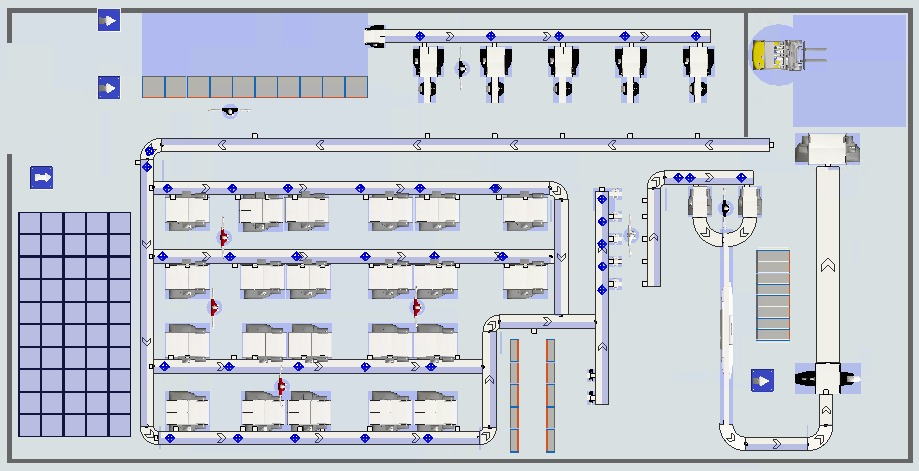
\includegraphics[scale=0.4]{../../Pictures/WhatsApp Image 2022-09-17 at 14.55.23.jpeg} 
\label{lay1}
\legend{Fonte: Autoria própria}
\end{center}
\end{figure}

\begin{figure}[H]
\begin{center}
\caption{Layout do chão de fábrica em detalhes}
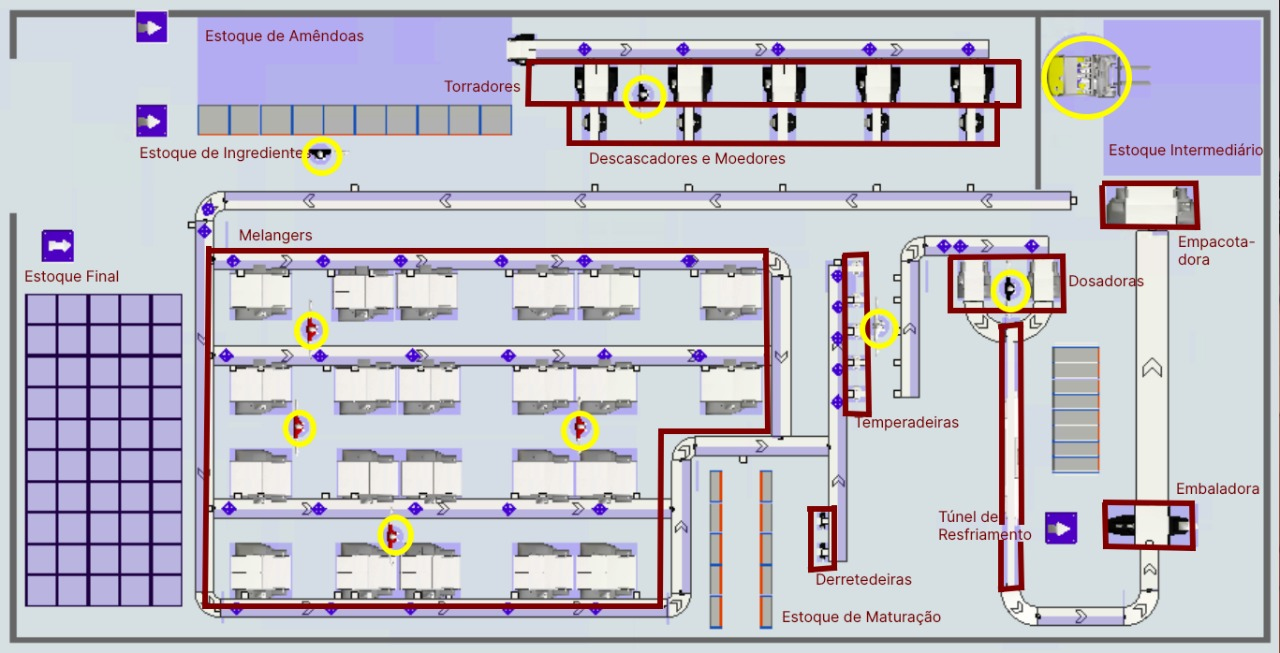
\includegraphics[scale=0.3]{../../Pictures/WhatsApp Image 2022-09-17 at 14.55.23 (1).jpeg} 
\label{lay2}
\legend{Fonte: Autoria própria}
\end{center}
\end{figure}

\newpage
\chapter{Tratamento de Efluentes}

A fábrica será instalada no estado de Minas Gerais, na cidade de Belo Horizonte. O licenciamento ambiental no município de Belo Horizonte é regido pela Lei Municipal N.º 7.277 de 17 de janeiro de 1997, regulamentada pelas Deliberações Normativas do Conselho Municipal de Meio Ambiente - DN 25/99 – normas específicas para atividades industriais.

De acordo com o artigo 4 desta lei:

Art. 4 - O licenciamento ambiental dos empreendimentos de médio porte mencionados nesta Deliberação Normativa terá a primeira etapa de licenciamento efetuada mediante a apresentação de Relatório de Controle Ambiental (RCA) e Plano de Controle Ambiental (PCA), segundo roteiro fornecido pela SMMA.

Dessa forma, para o licenciamento ambiental da fábrica será necessário a apresentação do Relatório de Controle Ambiental (RCA) e Plano de Controle Ambiental (PCA). 

O Relatório de Controle Ambiental (RCA) relata a conformidade ou não conformidade com relação ao atendimento das medidas mitigadoras e de controle ambiental. É exigido na fase de instalação ou de operação.

Devem ser considerados todos os aspectos potencialmente poluidores, como emissões atmosféricas e geração de resíduos e efluentes.

O Plano de Controle Ambiental (PCA) deve contemplar os projetos executivos de minimização de impactos avaliados na fase prévia.

Na fase de Licença de Instalação, tem foco de propor as medidas mitigadoras e de controle ambiental que o empreendedor deverá adotar para mitigar os impactos negativos e potencializar os impactos positivos decorrentes da instalação ou operação do empreendimento ou atividade. Define assim quais ações devem ser executadas para que a obra e a operação causem menor impacto possível ao meio ambiente.

Tendo em vista as exigências normativas citadas será necessário uma maior atenção nos pontos de tratamento de efluentes (não teremos emissão de gases poluentes na atmosfera) e impactos ambientais da operação, já que para instalação da fábrica não teremos nenhum impacto ambiental significativo.

Para o tratamento de efluentes, como já mencionado, teremos o tratamento dos efluentes líquidos, sólidos e de pós consumo.

Os efluentes líquidos consistem basicamente por resíduos de limpeza e esgoto
sanitário da empresa em geral. Por ser de pequeno porte, o destino dos efluentes líquidos é a rede de esgoto pública sem um tratamento prévio específico. Para ser lançada novamente a bacia hídrica, no entanto, faz-se necessário um tratamento pela instituição responsável. Nesse caso, como o efluente apresenta origem industrial torna-se indispensável um tratamento biológico devido às altas concentrações de matéria orgânica e nutrientes.

Os resíduos sólidos da indústria se dividem basicamente em produtos que serão
reprocessados, dejetos destinados aos aterros sanitários e de resíduos sólidos industriais e
materiais para reciclagem.

Os resíduos sólidos dos setores distintos da área produtiva são enviados para aterros
sanitários, por se tratarem de resíduos não perigosos segundo a classificação da norma
10004/2004 da ABNT \cite{ABNT}. Esses aterros são utilizados para a disposição de
resíduos sólidos urbanos no solo, sem causar danos à saúde pública e ao meio ambiente,
minimizando os impactos ambientais. Nesse caso, os resíduos são confinados na menor área
possível, reduzindo-os ao menor volume permissível, cobrindo-os com uma cama de terra
quando necessário. Esse método deve conter todos os elementos de proteção ambiental
\cite{FEAM}.

Em relação aos efluentes pós consumo e impactos ambientais da operação existe uma preocupação com o planejamento do ciclo de vida do produto e principalmente da embalagem, que visa garantir um destino para as embalagens dos chocolates em barra após o consumo. Para isso, ocorre a reciclagem do material polimérico, onde a estrutura do material residual é alterada, de modo que os subprodutos resultantes possam ser usados para outros fins que não a produção do material original, uma vez que em indústria de alimentos não se pode utilizar materiais reciclados.


\newpage
\chapter{Análise Financeira}

Com o intuito de verificar a viabilidade financeira da Showcolate! e do investimento que será realizado, foram levantados diversos gastos com utilidades, insumos, aluguel, mão de obra, maquinário e outros gastos menores. Além disso, também foi estipulados 15$\%$ do investimento total para eventuais imprevistos ou gastos não mapeados e um seguro de 10$\%$ para possíveis problemas relacionados com o capital de giro da empresa e o maquinário adquirido.

Para o cálculo dos insumos (Imagem \ref{1}) foram utilizados como base de cálculo os valores obtidos dos seguintes fornecedores: MFRural (Amêndoa de Cacau 5kg - R\$125,00) \cite{i1}, Guarani (Açúcar Refinado 25kg - R\$865,00) \cite{i2}, Ingredientes Online (Manteiga de Cacau 25kg - R\$1.185,00) \cite{i3}, FeijãoVeneza (Leite em Pó Integral 25kg - R\$906,00) \cite{i4} e Guangdong Changxing Printing Service Co., Ltd. (Rolo de BOPP para Embalagens FlowPack - R\$5,20/kg) \cite{i5}. E para o cálculo do peso das embalagens foi definido um valor de 10g de plástico para cada pacote de 100g. 

\begin{figure}[H]
\begin{center}
\caption{Gastos com insumos com base em 100$\%$ de produtividade - 2030}
\includegraphics[scale=0.5]{1.jpeg} 
\label{1}
\legend{Fonte: Autoria própria}
\end{center}
\end{figure}

Já as utilidades foram calculadas com base em valores da CEMIG (Companhia Energética de Minas Gerais) e COPASA (Companhia de Saneamento de Minas Gerais). Contudo, para o dimensionamento dos gastos foram realizadas estimativas com base em algumas notícias e conteúdos sobre agroindústrias, sendo que o gasto energético foi estimado também com base nas potências e períodos de uso das máquinas. \cite{ene} \cite{agua}

%\href{}{}

\begin{figure}[H]
\begin{center}
\caption{Gastos com utilidades}
\includegraphics[scale=0.55]{2.jpeg} 
\label{-}
\legend{Fonte: Autoria própria}
\end{center}
\end{figure}

O aluguel, como já mencionado anteriormente é referente a um galpão de 1000m² selecionado para comportar a empresa. Esse galpão se situa em Belo Horizonte e possui um aluguel de R\$17.000,00. \cite{galpao}

\begin{figure}[H]
\begin{center}
\caption{Gasto com aluguel}
\includegraphics[scale=0.55]{3.jpeg} 
\label{-}
\legend{Fonte: Autoria própria}
\end{center}
\end{figure}

No caso da mão de obra, foram dimensionadas as necessidades de acordo com o tamanho da produção planejada e o organograma da empresa. As áreas de apoio foram pensadas seguindo o modelo de negócios e as necessidades específicas da empresa.

Na figura abaixo trazemos os cargos e as quantidades necessárias de funcionários, contando com a mão de obra direta e indireta e áreas administrativas, bem como os gastos correspondentes com salários e encargos. Os salários foram cotados de acordo com o parâmetro de salários encontrados para as vagas de diretor industrial e operador de máquinas e levando em consideração as leis trabalhistas para o cálculo dos encargos, ou seja, um percentual de aproximadamente 70$\%$ de encargos que já está adicionado nos gastos cotados abaixo de salários. \cite{sala1} \cite{sala2} \cite{encargos}


\begin{figure}[H]
\begin{center}
\caption{Gasto com mão de obra}
\includegraphics[scale=0.6]{4.jpeg} 
\label{-}
\legend{Fonte: Autoria própria}
\end{center}
\end{figure}


Os maquinários foram precificados de acordo com os fornecedores encontrados a seguir: Inove máquinas industriais \cite{m1}, Amantes da Breja \cite{m2}, Zhengzhou Longer Machinery Co., Ltd. \cite{m3}, Chocolate Melangeur \cite{m4}, CENCIFABRISGIOVAN \cite{m5}, Vonin \cite{m6}, Cetro Máquinas - Envasadora \cite{m7}, Vibramax \cite{m8} e Cetro Máquinas - FlowPack Invertida \cite{m9}. Apenas o túnel de resfriamento que não foi possível encontrar um valor mais exato já que não foi encontrado um anúncio com valor e para conseguir um orçamento seria necessário entrar em contato com fornecedores para tal. Logo, foi estipulado um valor com base no custo dos outros equipamentos.


\begin{figure}[H]
\begin{center}
\caption{Investimento em maquinário}
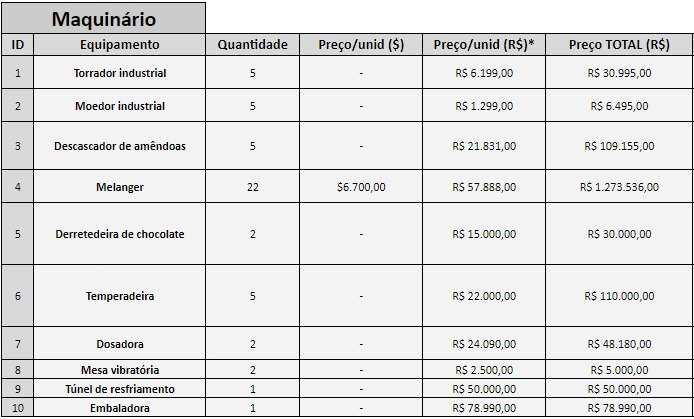
\includegraphics[scale=0.6]{5.jpeg} 
\label{-}
\legend{Fonte: Autoria própria}
\end{center}
\end{figure}

\section{Investimento}

Aqui foram listados gastos principalmente não recorrentes que serão necessários para a implantação da indústria e para dar início à operação. 

Além disso, foi considerado a depreciação esperada para esses itens, tendo em vista que são ativos com alto valor e depreciam com o passar do tempo.

Os cálculos foram feitos trazendo duas opções, o capital de giro anual e trimestral. Isso permite com que possamos ponderar os dois resultados e escolher o financiamento de capital de giro com melhor retorno para o negócio.

\begin{figure}[H]
\begin{center}
\caption{Investimento total e depreciação}
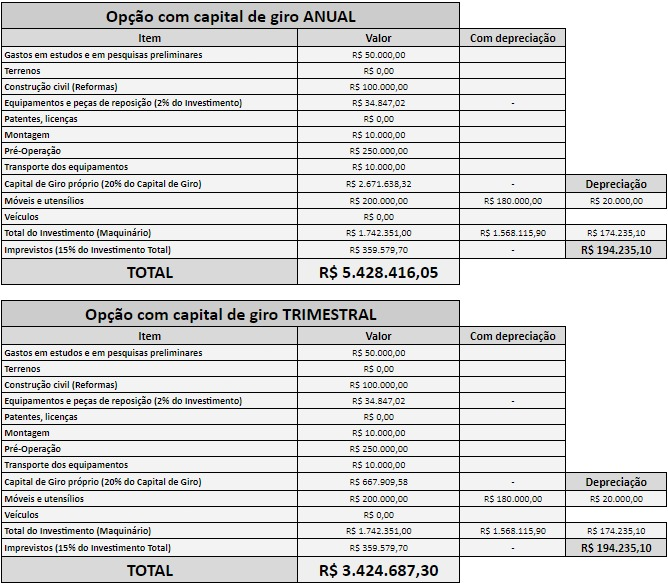
\includegraphics[scale=0.7]{a1.jpeg} 
\label{-}
\legend{Fonte: Autoria própria}
\end{center}
\end{figure}

\section{Custeio}

Para realizar o custeio separado por produto foi utilizado os valores dos insumos (já mencionados anteriormente) multiplicados pela produção esperada.

Todos os custos indiretos foram rateados entre os diferentes produtos usando como parâmetro a representatividade do produto sobre a produção total. Assim foi encontrado o custo unitário dos produtos e aplicado uma porcentagem para formação do preço de venda. 

\begin{figure}[H]
\begin{center}
\caption{Custeio dos tabletes de 100g de cada tipo de chocolate - 2024}
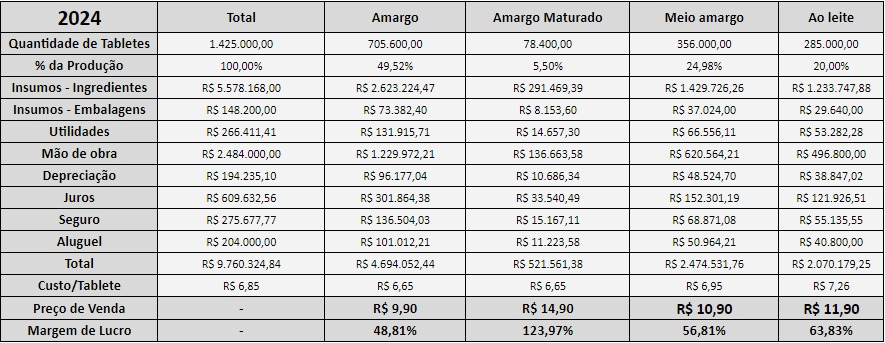
\includegraphics[scale=0.4]{a2.jpeg} 
\label{-}
\legend{Fonte: Autoria própria}
\end{center}
\end{figure}

\section{Financiamento}

Para a fazer a empresa começar a rodar e comprar os equipamentos e pagar as contas iniciais foram realizadas as projeções de 2 financiamentos. Sendo o primeiro relacionado com 80$\%$ do capital de giro (Imagem \ref{fin1}) enquanto o segundo financiamento é relacionado com o investimento total da empresa somado a 20$\%$ do capital de giro (Imagem \ref{fin2}), que seria o investimento próprio. Dessa forma, não está planejado o uso de investimento próprio, já que ambos os financiamentos cobrem 100$\%$ do valor necessário. Além disso, é importante citar que o capital de giro utilizado nos cálculos é referente a um trimestre de 2030, o ano em que a fábrica estará produzindo 100$\%$ da sua capacidade. As taxas utilizadas para a simulação dos financiamentos foi de 10$\%$ e em ambos foi adicionado 2 anos de carência.

\begin{landscape}

\begin{figure}[]
\begin{center}
\caption{Financiamento do Investimento}
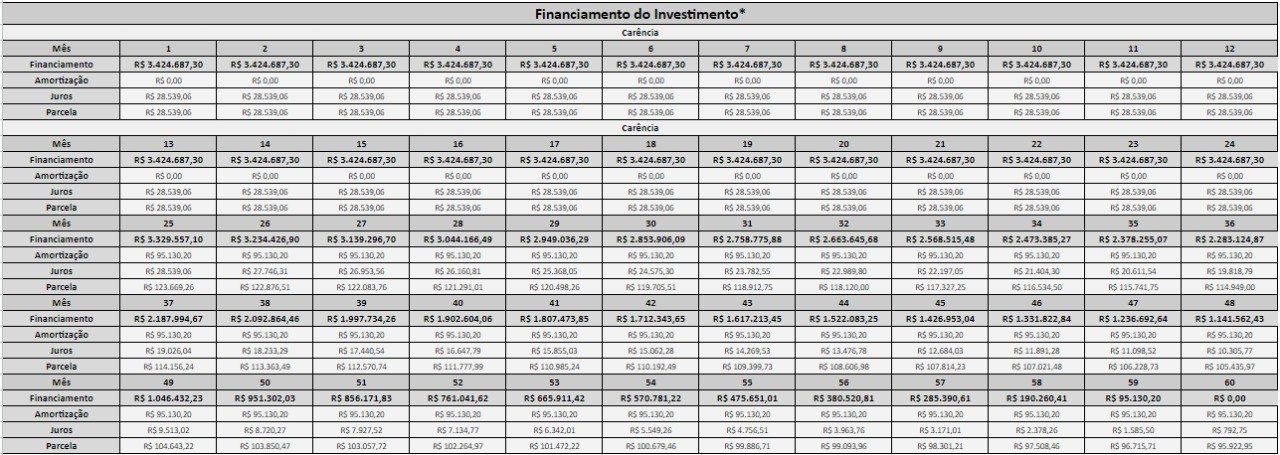
\includegraphics[scale=0.5]{a3.jpeg} 
\label{fin1}
\legend{Fonte: Autoria própria}
\end{center}
\end{figure}

\end{landscape}

\begin{landscape}

\begin{figure}[]
\begin{center}
\caption{Financiamento do Capital de Giro}
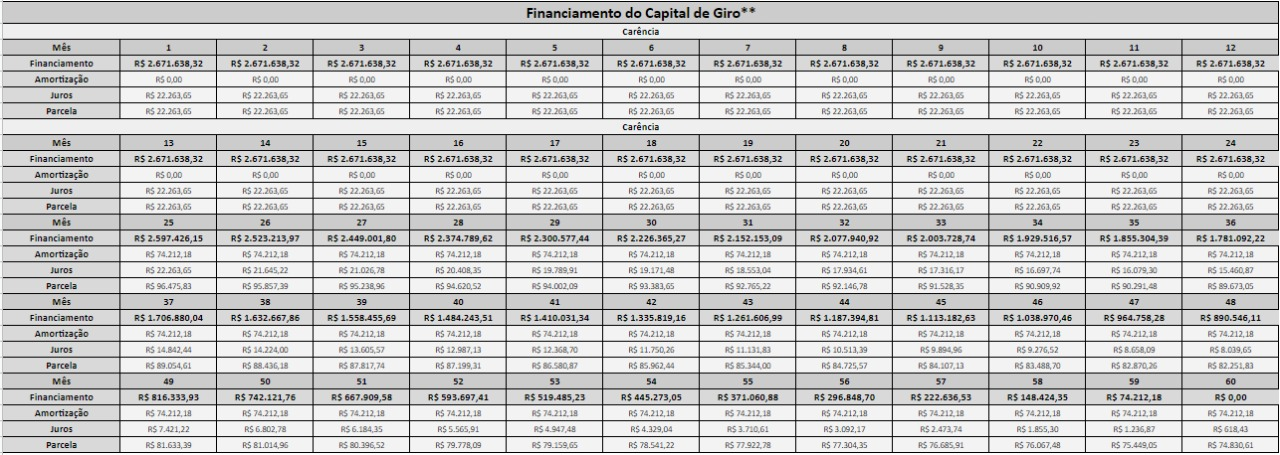
\includegraphics[scale=0.5]{a4.jpeg} 
\label{fin2}
\legend{Fonte: Autoria própria}
\end{center}
\end{figure}

\end{landscape}

\section{Demonstração de Resultados}

Para a obtenção do demonstrativo de resultados da empresa foram mapeados os impostos, calculados os faturamentos de cada ano, segundo o valor de venda de cada chocolate e estruturados todos os custos e despesas que ocorrem durante a produção.

São 6 impostos desde a produção até a distribuição do chocolate e a chegada do mesmo ao consumidor final. É importante frisar que o ICMS, PIS, COFINS e IPI são aplicáveis na dedução da receita bruta e o restante são aplicados sobre o resultado operacional líquido. Além disso, foi adicionada uma reserva de impostos no valor de 0,5$\%$ que está sendo calculada sobre a receita bruta para cobrir eventuais falhas relacionadas aos cálculos dos impostos. \ref{imp1} \ref{imp2} \ref{imp3} \ref{imp4} \ref{imp5}

\begin{figure}[H]
\begin{center}
\caption{Alíquotas de impostos relacionadas a produção de chocolate}
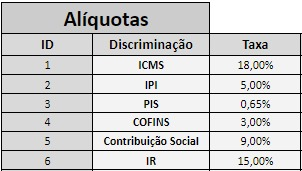
\includegraphics[scale=0.5]{a5.jpeg} 
\label{-}
\legend{Fonte: Autoria própria}
\end{center}
\end{figure}

A estrutura do DRE  se faz a partir da receita bruta, Receita operacional líquida, onde vai se reduzir os custos das vendas e se obter o resultado operacional bruto, que por sua vez será deduzido as despesas operacionais encontrando assim o EBITDA (Earnings Before Interest, Taxes, Depreciation and Amortization), em que vai se deduzir a depreciação ou amortização dessa forma obtendo-se o EBT (Earnings Before Interest and Taxes), onde vai se deduzir os juros e imposto de renda se encontrando finalmente o resultado líquido do exercício.

Na Imagem \ref{dre} é possível verificar todos os campos listados acima e também os valores crescentes do Resultado Líquido, que era previsto por causa da demanda mensurada anteriormente. E na Imagem \ref{dre2}, é possível analisar melhor os detalhes da estrutura.

\begin{landscape}

\begin{figure}[]
\begin{center}
\caption{Demonstração do Resultado do Exercício - Projeção Anual}
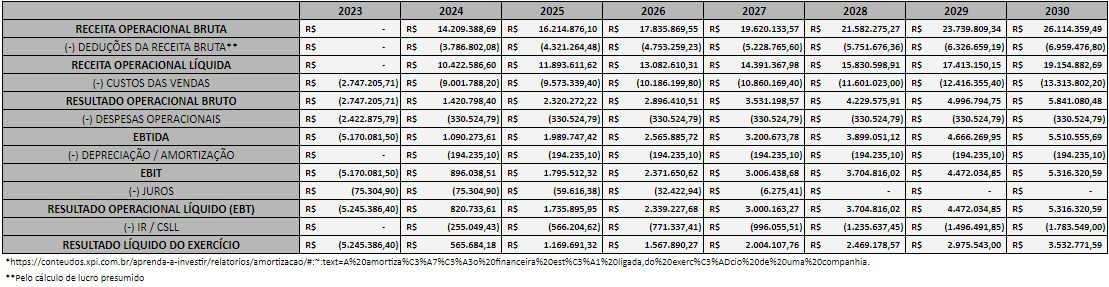
\includegraphics[scale=0.6]{a6.jpeg} 
\label{dre}
\legend{Fonte: Autoria própria}
\end{center}
\end{figure}

\end{landscape}

\begin{landscape}

\begin{figure}[]
\begin{center}
\caption{Demonstração do Resultado do Exercício - Projeção Anual - Detalhada}
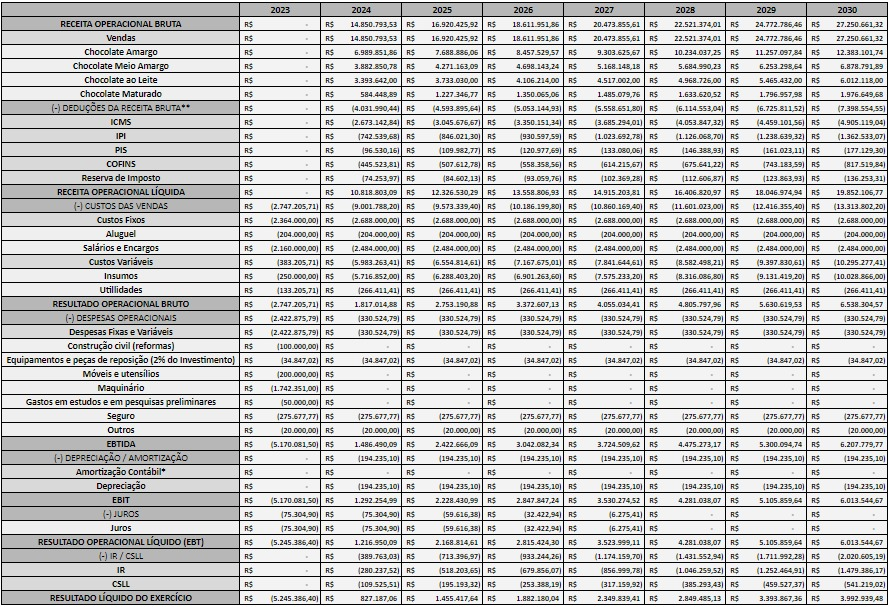
\includegraphics[scale=0.7]{a8.jpeg} 
\label{dre2}
\legend{Fonte: Autoria própria}
\end{center}
\end{figure}

\end{landscape}

\section{Cronograma Financeiro e Indicadores}

O cronograma financeiro, diferente do DRE, possui o gasto com a amortização financeira, que é relacionada com os pagamentos dos financiamentos. Além disso, também é possível verificar a variação macro que ocorre no caixa da empresa adicionando a entrada do financiamento no primeiro ano e acumulando os resultados dos caixas dos anos seguintes, como é possível verificar na Imagem \ref{cro}. 

Com a ajuda do cronograma é possível construir os seguintes gráficos:

\begin{figure}[H]
\begin{center}
\caption{Resultado Líquido do Exercício + Amortização Financeira}
\includegraphics[scale=0.35]{a10.png} 
\label{a10}
\legend{Fonte: Autoria própria}
\end{center}
\end{figure}

\begin{figure}[H]
\begin{center}
\caption{Projeção Macro Anual do Fluxo de Caixa da Showcolate!}
\includegraphics[scale=0.35]{a11.png} 
\label{a11}
\legend{Fonte: Autoria própria}
\end{center}
\end{figure}

\begin{landscape}

\begin{figure}[]
\begin{center}
\caption{Demonstração do Resultado do Exercício - Projeção Anual - Detalhada}
\includegraphics[scale=0.55]{a9.jpeg} 
\label{cro}
\legend{Fonte: Autoria própria}
\end{center}
\end{figure}

\end{landscape}

\subsection{Payback}

E com os dados do cronograma também é possível analisar o payback da empresa. Sendo o investimento da Showcolate!, todo o valor gasto no ano de 2023, houve um investimento de R\$5.245.386,40; e esse valor só é recuperado no ano de 2029, ou seja, 7 anos de payback, como é possível verificar no gráfico da Imagem \ref{pay}. Esse gráfico foi estruturado com o Lucro Líquido da Showcolate! sendo o começo de cada ano o resultado do Lucro Líquido do ano anterior, assim ocorre uma acumulação do Lucro Líquido que faz com que possamos observar o payback, ou seja, o período em que o investimento inicial é recuperado.

\begin{figure}[H]
\begin{center}
\caption{Payback da Showcolate!}
\includegraphics[scale=0.28]{a12.png} 
\label{pay}
\legend{Fonte: Autoria própria}
\end{center}
\end{figure}

\subsection{Ponto de Equilíbrio}

E outro indicador muito importante é o Ponto de Equilíbrio, que no caso da Showcolate! irá indicar quantas unidades de 100g precisam ser vendidas para que a empresa não tenha prejuízo. Para encontrar o valor desse indicador foi plotado um gráfico e verificado os valores das intersecções das retas de faturamento com as retas de gasto fixo, e gastos fixos + variáveis. Na Imagem \ref{pq} é possível visualizar as intersecções que ocorrem no gráfico.


\begin{figure}[H]
\begin{center}
\caption{Ponto de Equilíbrio da Showcolate! - 2024} 
\includegraphics[scale=0.3]{a13.png} 
\label{pq}
\legend{Fonte: Autoria própria}
\end{center}
\end{figure}


Para calcular os pontos exatos foram igualadas as equações das retas e como a Showcolate! possui diversos tipos de produtos, foi aplicada a proporção entre todos eles para obter o preço de venda médio, que é de R\$10,42 para ser utilizado nos cálculos. 

Assim, o ponto de equilíbrio do ano de 2024 para os gastos fixos gira em torno de 309.384, enquanto o ponto de equilíbrio para os gastos fixos + variáveis gira em torno de 538.432. Portanto, seguindo a proporção para os diferentes tipos de chocolates, seriam necessários vender em torno de 266.609 chocolates amargos, 29.623 chocolates maturados, 134.514 chocolates meio amargos e 107.686 chocolates ao leite, para a obtenção do ponto de equilíbrio relacionado com os gastos fixos + variáveis.


Por fim, é possível resumir a análise financeira na Imagem \ref{res}. 

\begin{figure}[H]
\begin{center}
\caption{Resumo da Análise Financeira}
\includegraphics[scale=0.7]{a11.jpeg} 
\label{res}
\legend{Fonte: Autoria própria}
\end{center}
\end{figure}

\newpage
\chapter{Conclusão}
%\pagestyle{fancy}

No decorrer deste estudo sobre o processamento de cacau verificou-se a importância dos cálculos de balanço de massa e balanço de energia para dimensionamento da linha de produção. Já que dessa forma é possível analisar a capacidade da linha de produção por meio das perdas que acontecem no sistema, o gasto energético de todos os equipamentos e também o dimensionamento correto do maquinário igual como ocorreu com o túnel de resfriamento da linha de produção deste trabalho.

Além disso, foi possível analisar o mercado, as normas e leis regulamentadoras do setor do chocolate e entender todo o processo de produção desse produto, o que ocasionou em um grande aprendizado sobre o setor e sobre o dimensionamento de uma fábrica. Ademais, foi realizado um estudo acerca dos resíduos e foram calculados todas as perdas que ocorrem na produção e toda a energia que é consumida na linha de fabricação do chocolate.

Com a definição de uma marca, a criação de valores e a estruturação dos produtos, foi possível verificar o quanto são difíceis as escolhas que os empresários precisam realizar, já que detalhes podem resultar em grandes alterações financeiras. Entre essas escolhas está a definição da localização da fábrica, a capacidade produtiva que ela terá, a forma como deverão ser posicionados os maquinários para obter a melhor eficiência, assim como a escolha dos melhores fornecedores.

Por fim, a análise financeira por mais complexa que seja é de demasiada importância. Como já mencionado, mudanças mínimas no projeto podem resultar em grandes economias e podem fazer muita diferença para a competitividade da marca no mercado. Muitos custos e gastos não foram dimensionados com tanto detalhamento, contudo já foi possível analisar o quanto os impostos impactam nos resultados e também na média de tempo que normalmente demora para empresas semelhantes atingirem o payback.

Esse trabalho exploratório ampliou a visão sobre a complexidade de dimensionar uma empresa e também sobre como funciona o processamento de cacau e a fabricação de chocolates. Ademais, o papel do engenheiro de produção ficou ainda mais claro como sendo algo essencial, já que a maioria desses dimensionamentos necessitam de precisão e técnicas.


\newpage
\postextual


\bibliography{referencias}

\begin{anexosenv}

\chapter{Propriedades na Saturação - REFRIGERANTE R-717 (AMÔNIA)}

\begin{figure}[H]
\begin{center}
%\caption{Balanço de Energia - Chocolate Ao Leite}
\includegraphics[scale=1.1]{../../Pictures/tabelaamonia.png} 
%\legend{Fonte: Autoria Própria}
\end{center}
\end{figure}

\chapter{Diagrama p-h - REFRIGERANTE R-717 (AMÔNIA)}

\begin{figure}[H]
\begin{center}
%\caption{Balanço de Energia - Chocolate Ao Leite}
\includegraphics[scale=1.12]{../../Pictures/graficoamonia.png} 
%\legend{Fonte: Autoria Própria}
\end{center}
\end{figure}

%\begin{lstlisting}
%\end{lstlisting}

\end{anexosenv}

\end{document}
